\documentclass[14pt]{article}
\topmargin -0.7in
\oddsidemargin -0.21in
\evensidemargin -0.21in
\textwidth=17cm
\textheight=24cm

\usepackage[utf8]{inputenc}
\usepackage[T2A]{fontenc} 
\usepackage[russian]{babel}
\usepackage{amsmath}
\usepackage{comment}

\usepackage{tikz}
\usepackage{graphicx}
\graphicspath{{./jpeg/}}
\DeclareGraphicsExtensions{.jpg}

\renewcommand{\l}{\left( }
\renewcommand{\r}{\right) }
\renewcommand{\phi}{\varphi}
\newcommand{\pd}{\partial}
\newcommand{\br}[1]{\l {#1} \r}
\newcommand{\rint}{\int\limits_{-\infty}^{+\infty}}
\newcommand{\pint}{\int\limits_{-\pi}^{\pi}}
\newcommand{\jacobian}[2]{\frac{\pd \br{#1}}{\pd \br{#2}}}
\newcommand{\abs}[1]{\left| #1 \right|}
\renewcommand{\line}{\\ \_\_\_\_\_\_\_\_\_\_\_\_\_\_\_\_\_\_\_\_\_\_\_\_\_\_\_\_\_\_\_\_\_\_\_\_\_\_\_\_\_\_\_\_\_\_\_\_\_\_\_\_\_\_\_\_\_\_\_\_\_\_\_ \\ }

\begin{document}
% 1 - 3
$$$$
$$$$
$$$$
$$$$

\begin{minipage}[h]{0.5\linewidth}

\includegraphics[width=1\linewidth]{page-01.jpg}
\end{minipage}
\begin{minipage}[h]{0.45\linewidth}
\center{Представиться.}
\end{minipage}
\line

\begin{minipage}[h]{0.5\linewidth}
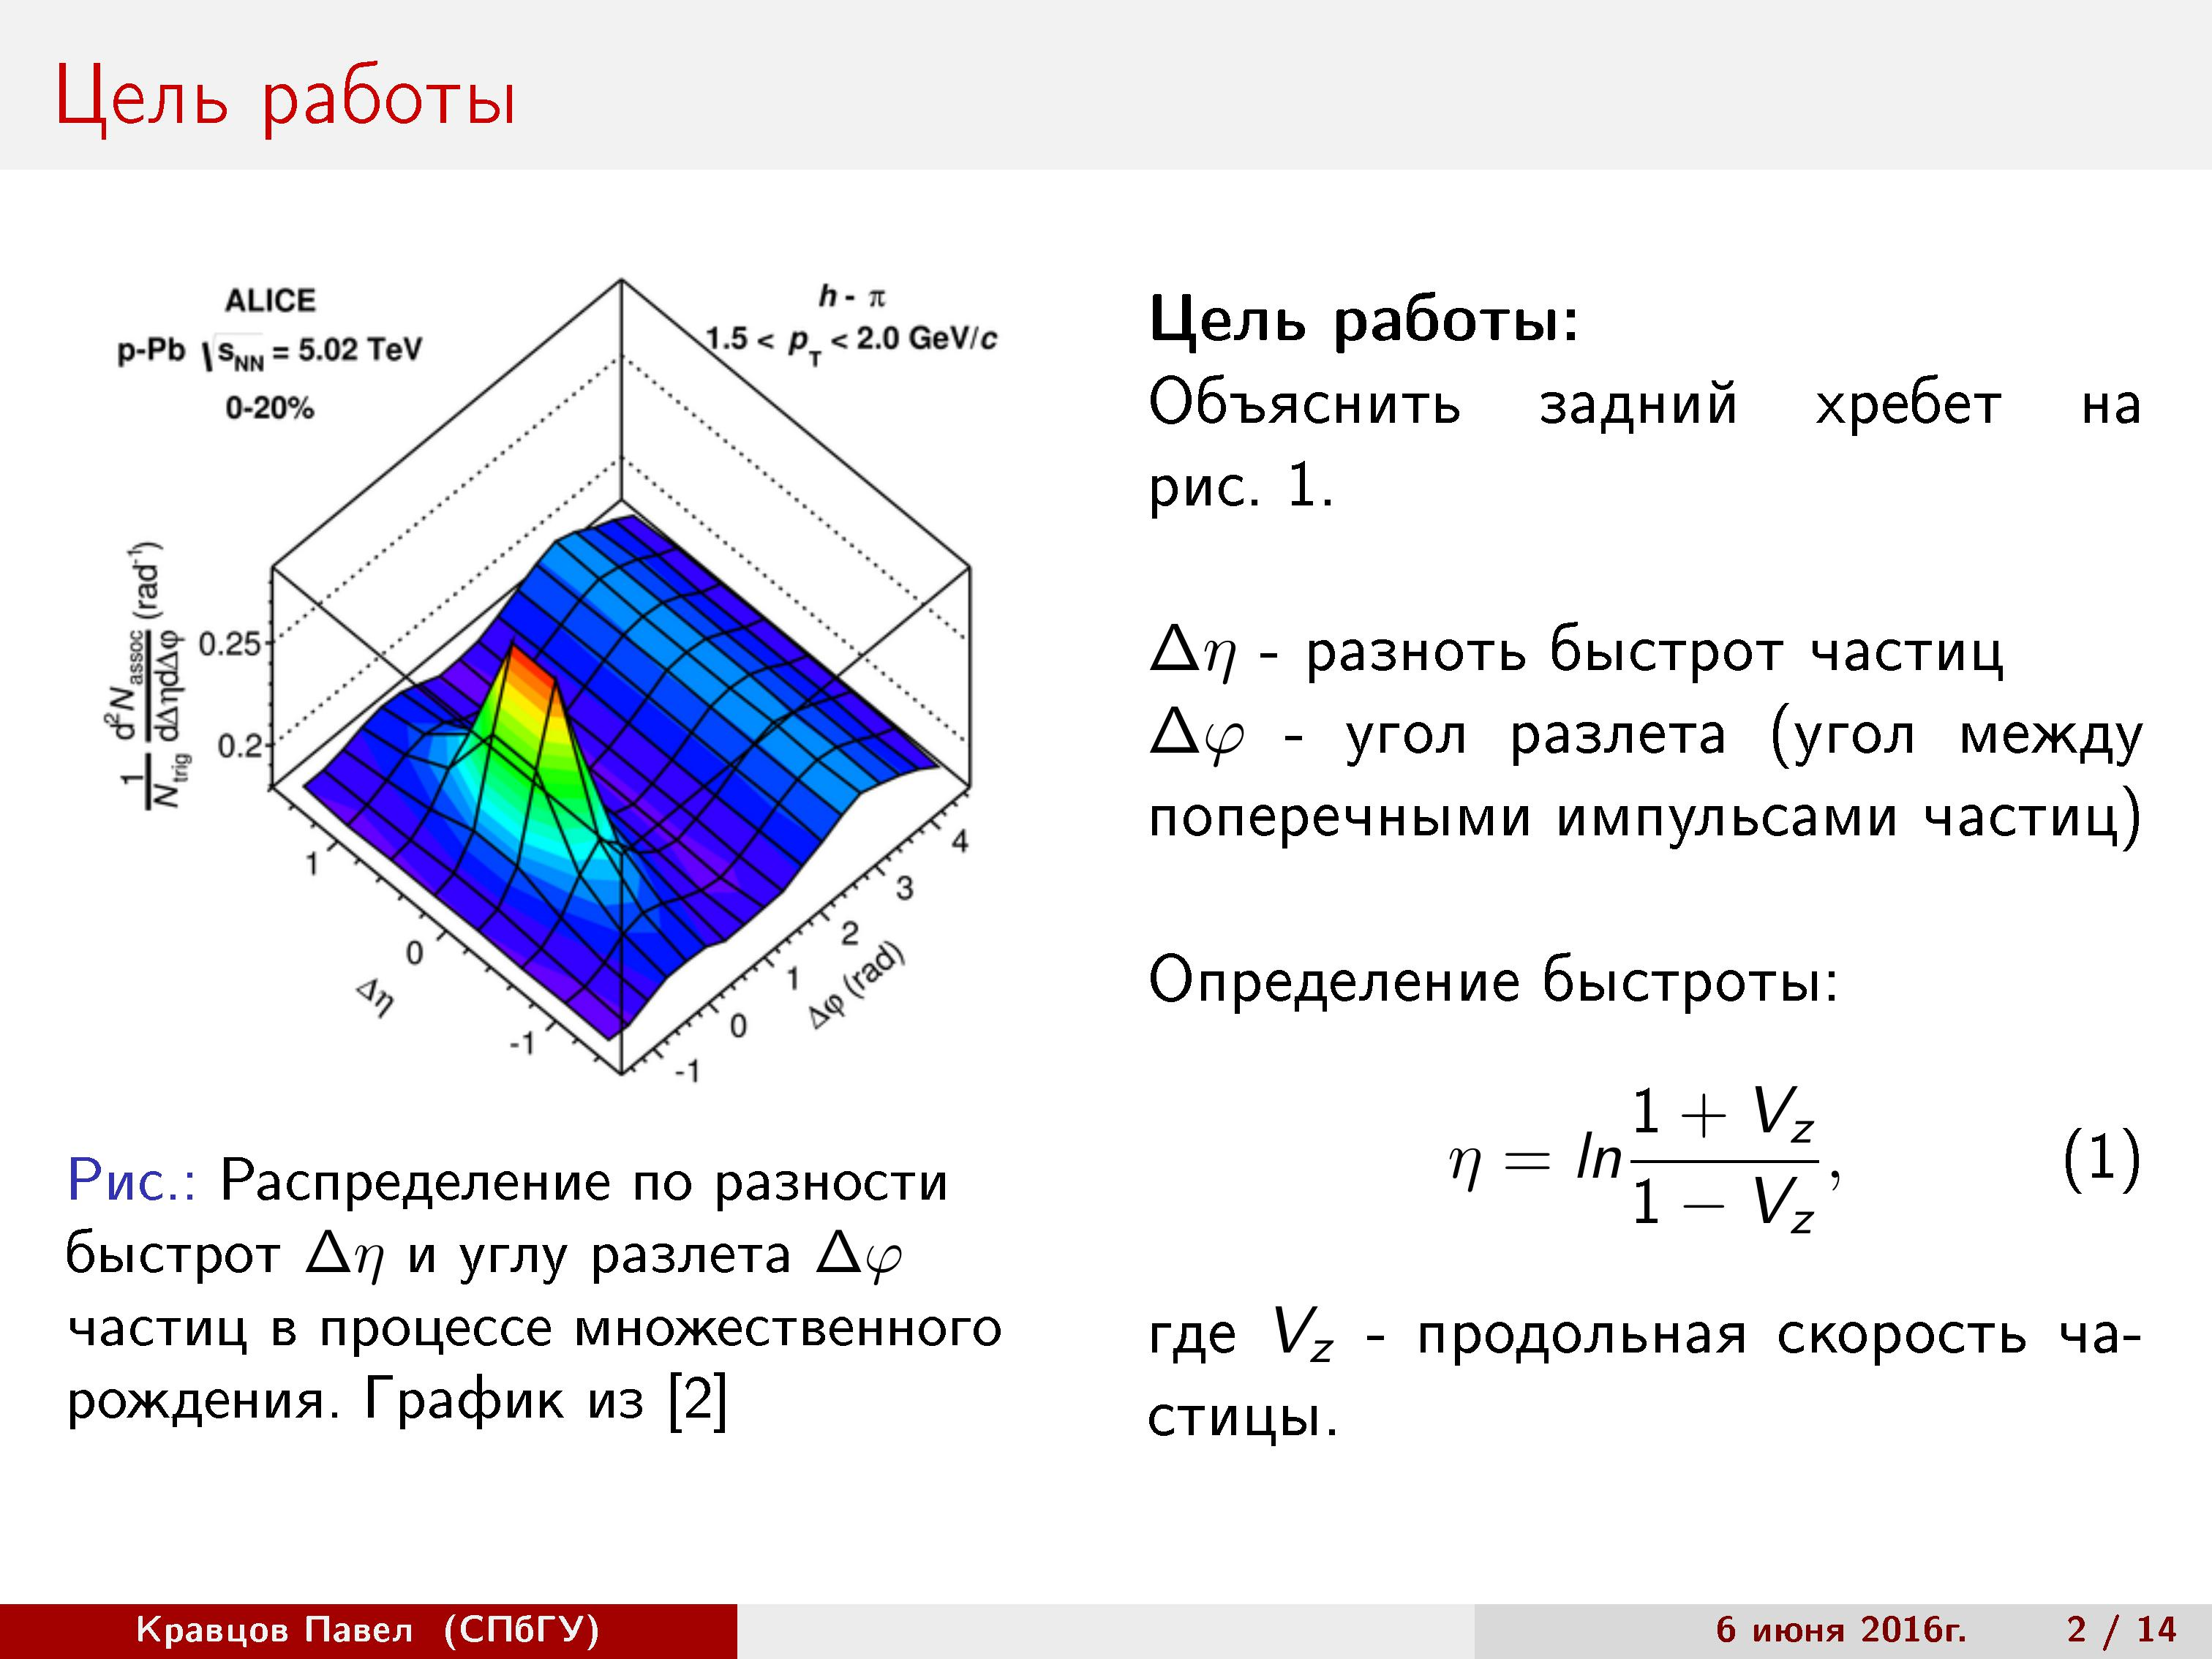
\includegraphics[width=1\linewidth]{page-02.jpg}
\end{minipage}
\begin{minipage}[h]{0.45\linewidth}
В адроных столкновениях часто изучается статистика столкновений по быстроте и углу разлета образовавшихся частиц. Быстрота - это функция продольной скорости частиц (см. формулу), угол разлета - угол между поперечными импульсами частиц. Это характерное распределение числа частиц по быстроте и углу разлета, полученное из эксперимента. Его также называют 2-х частичной корреляционной функцией.

Целью нащей работы является объяснение в рамках струнного подхода вот этого заднего хребта, или как его называют, заднего риджа на рисунке. Передний пик уже имеет объяснение, позже мы его упомянем.
\end{minipage}
\line

\begin{minipage}[h]{0.5\linewidth}
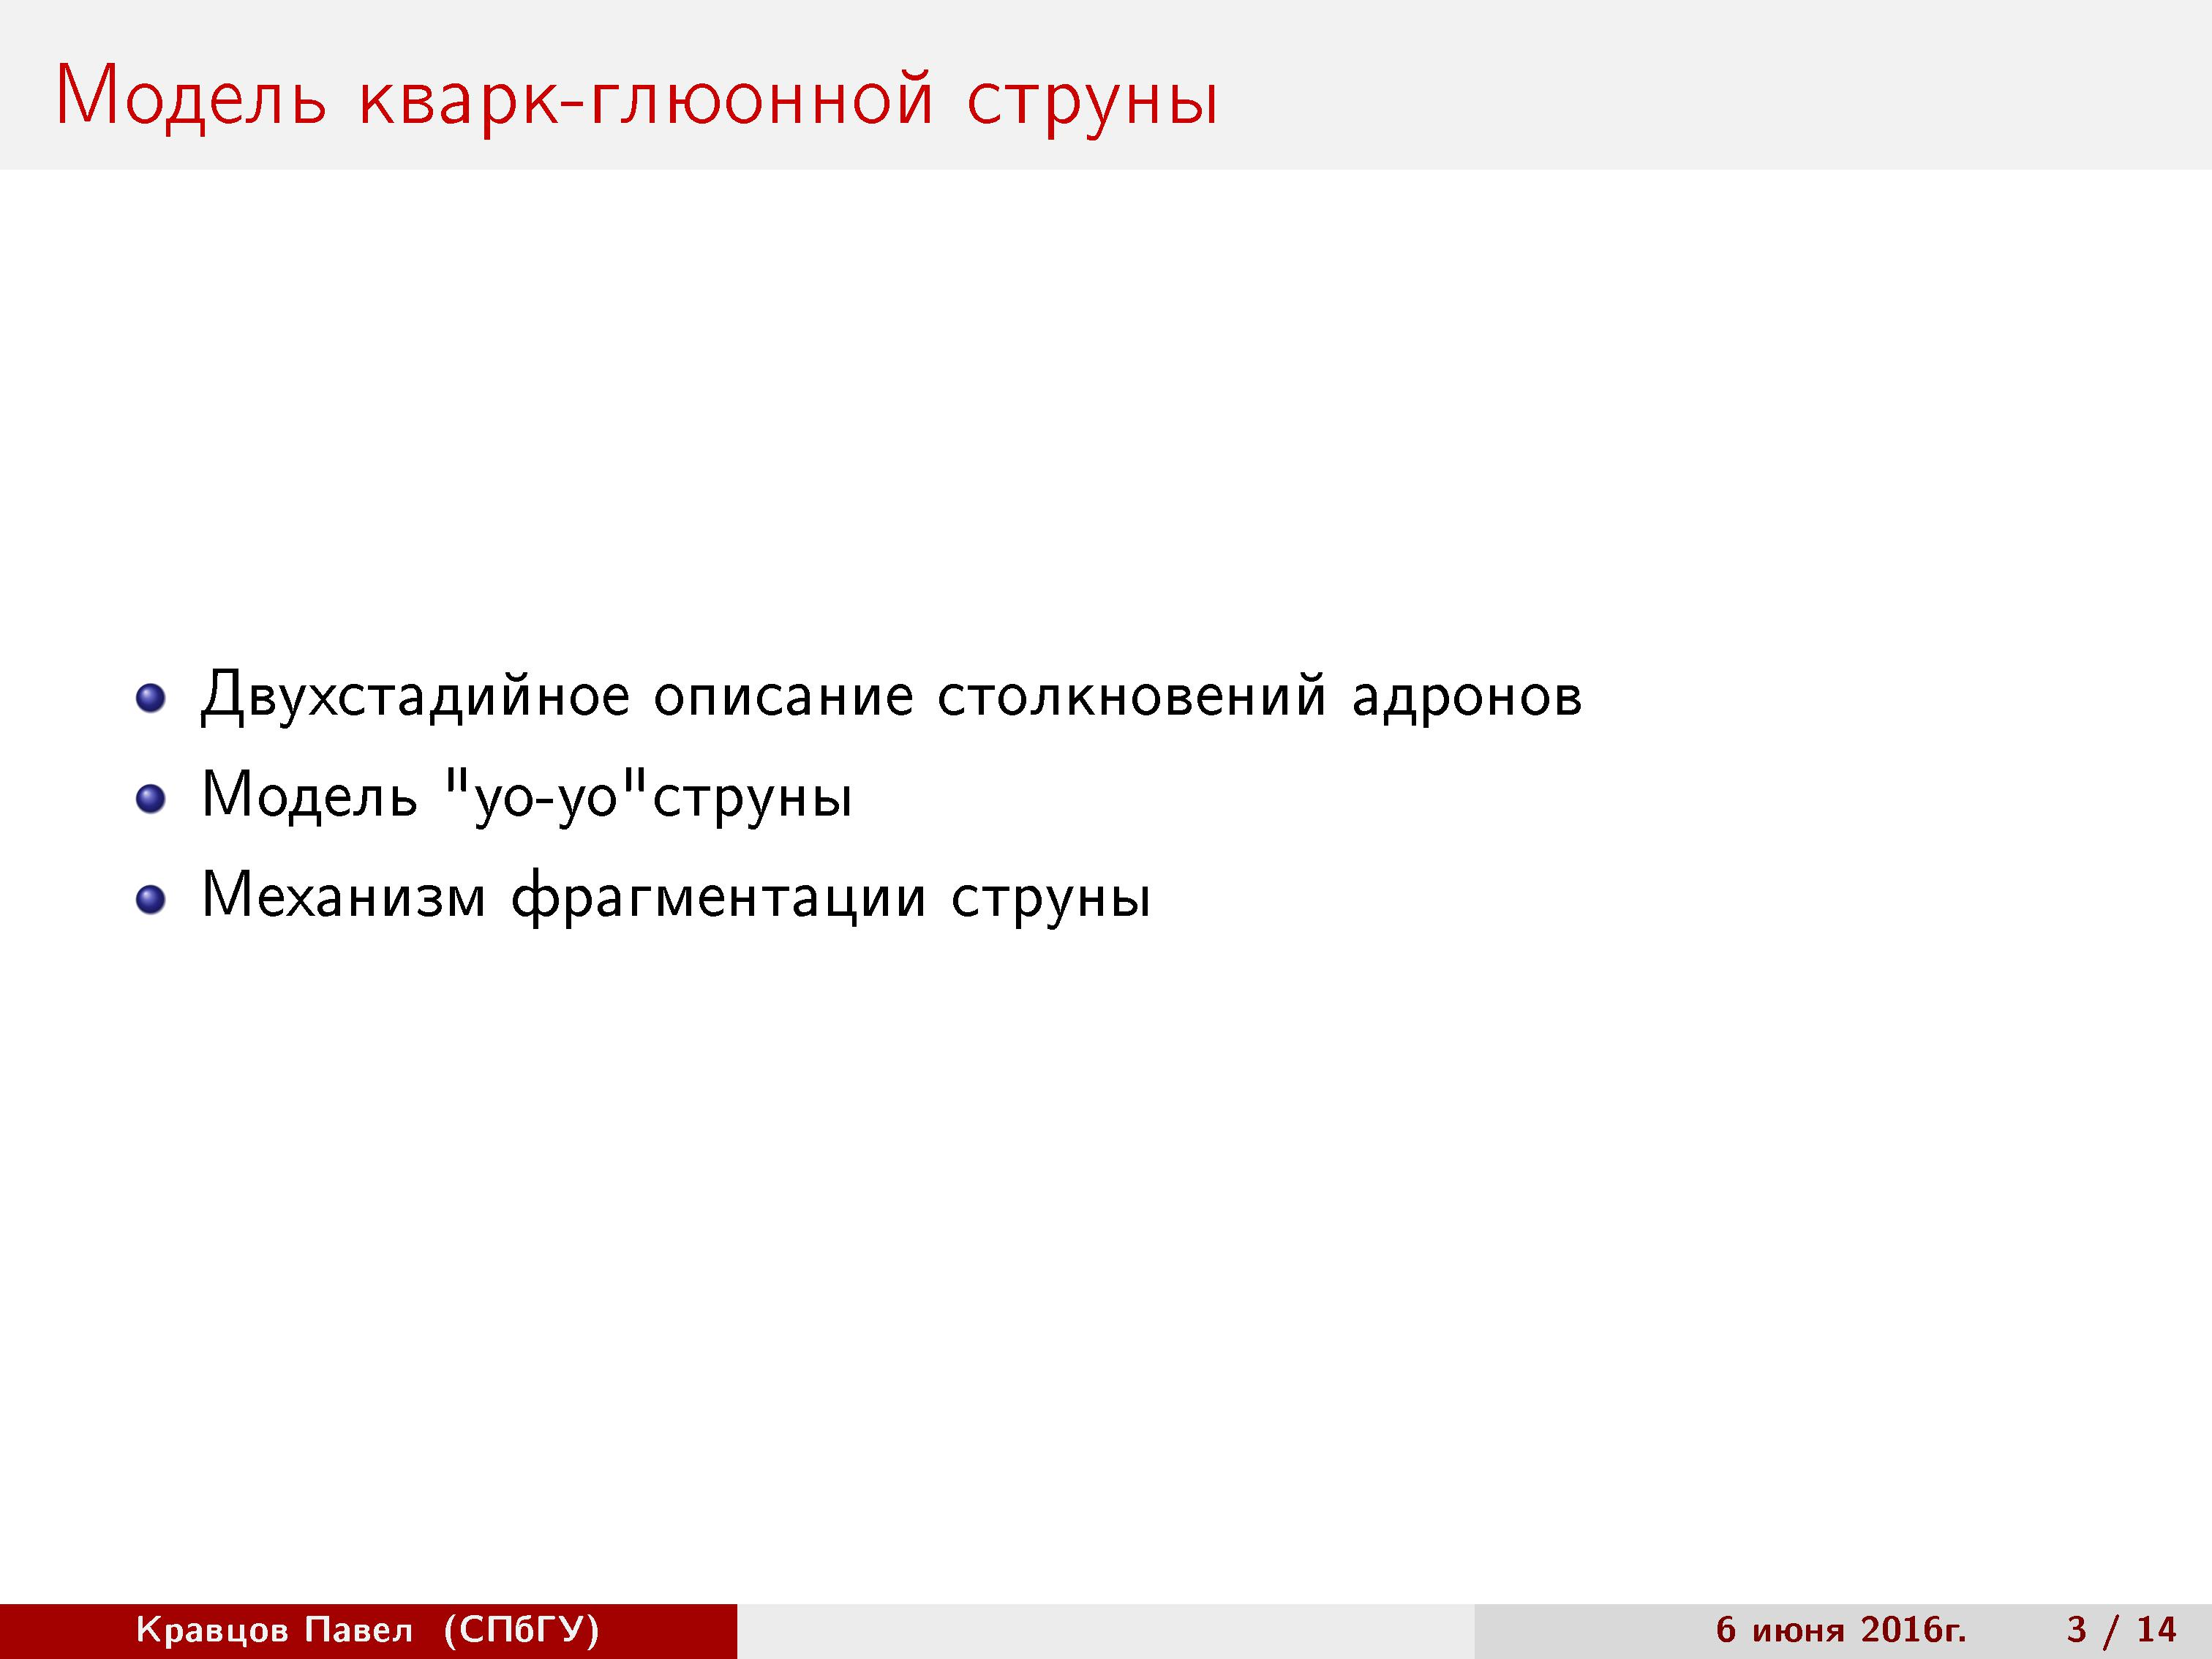
\includegraphics[width=1\linewidth]{page-03.jpg}
\end{minipage}
\begin{minipage}[h]{0.45\linewidth}
Для начала обсудим, в чем состоит струнный подход для описания адронных столкновений. Он включает в себя некоторые феноменологические модели и механизмы. Нам понадобятся эти три.
Рассмотрим их подробнее.
\end{minipage}
\line

% 4 - 6
\newpage
$$$$
$$$$
$$$$
$$$$

\begin{minipage}[h]{0.5\linewidth}
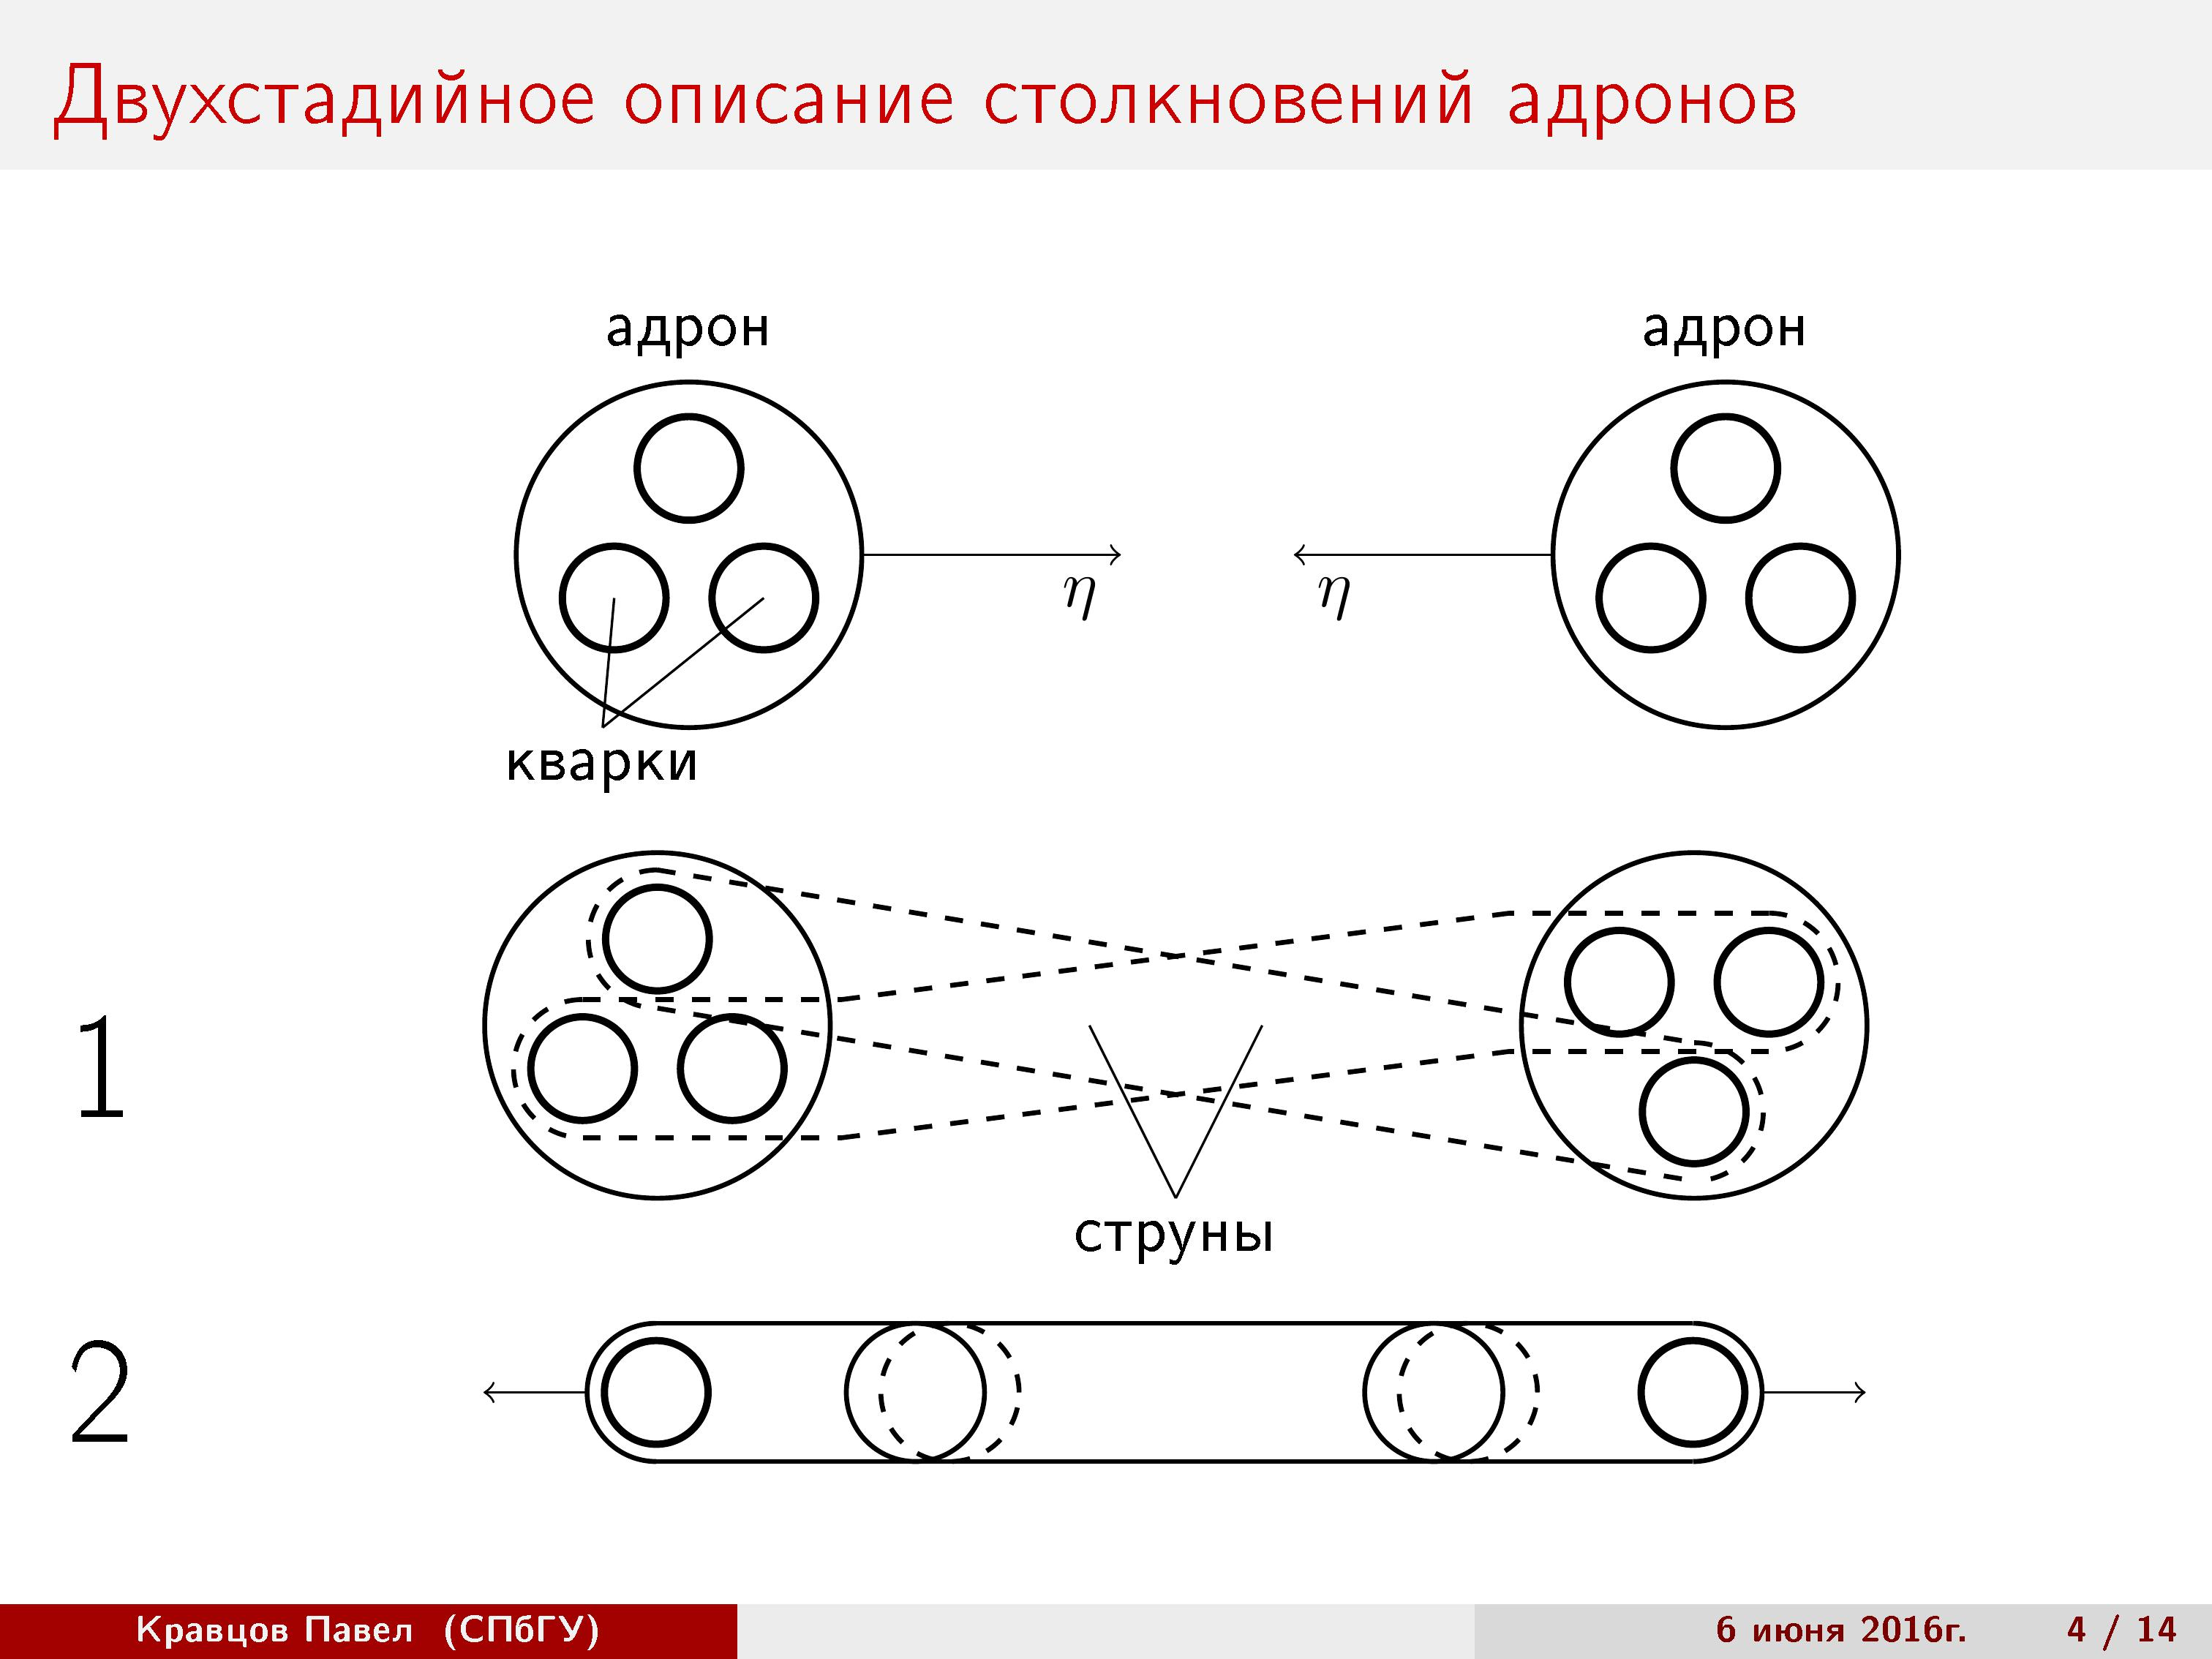
\includegraphics[width=1\linewidth]{page-04.jpg}
\end{minipage}
\begin{minipage}[h]{0.45\linewidth}
Сначала обсудим откуда появляются струны.

В ускорителе, друг навстречу другу летят адроны с околосветовой скоростью, т. е. с большой быстротой. Вначале считается, что кварки в адронах взаимодействуют только с кварками из своего адрона. При столкновении, цветовые поля из кварков перецепляются на другие кварки и бикварки. Эти поля ведут себя как струны. Потом эти струны рвуться и образуется множество новых струн-частиц.

Такое феноменологическое описание называется двухстадийным описанием. Перецепление полей и образование струн - 1 стадия. Разрыв, или фрагментация струн - 2 стадия.
\end{minipage}
\line

\begin{minipage}[h]{0.5\linewidth}
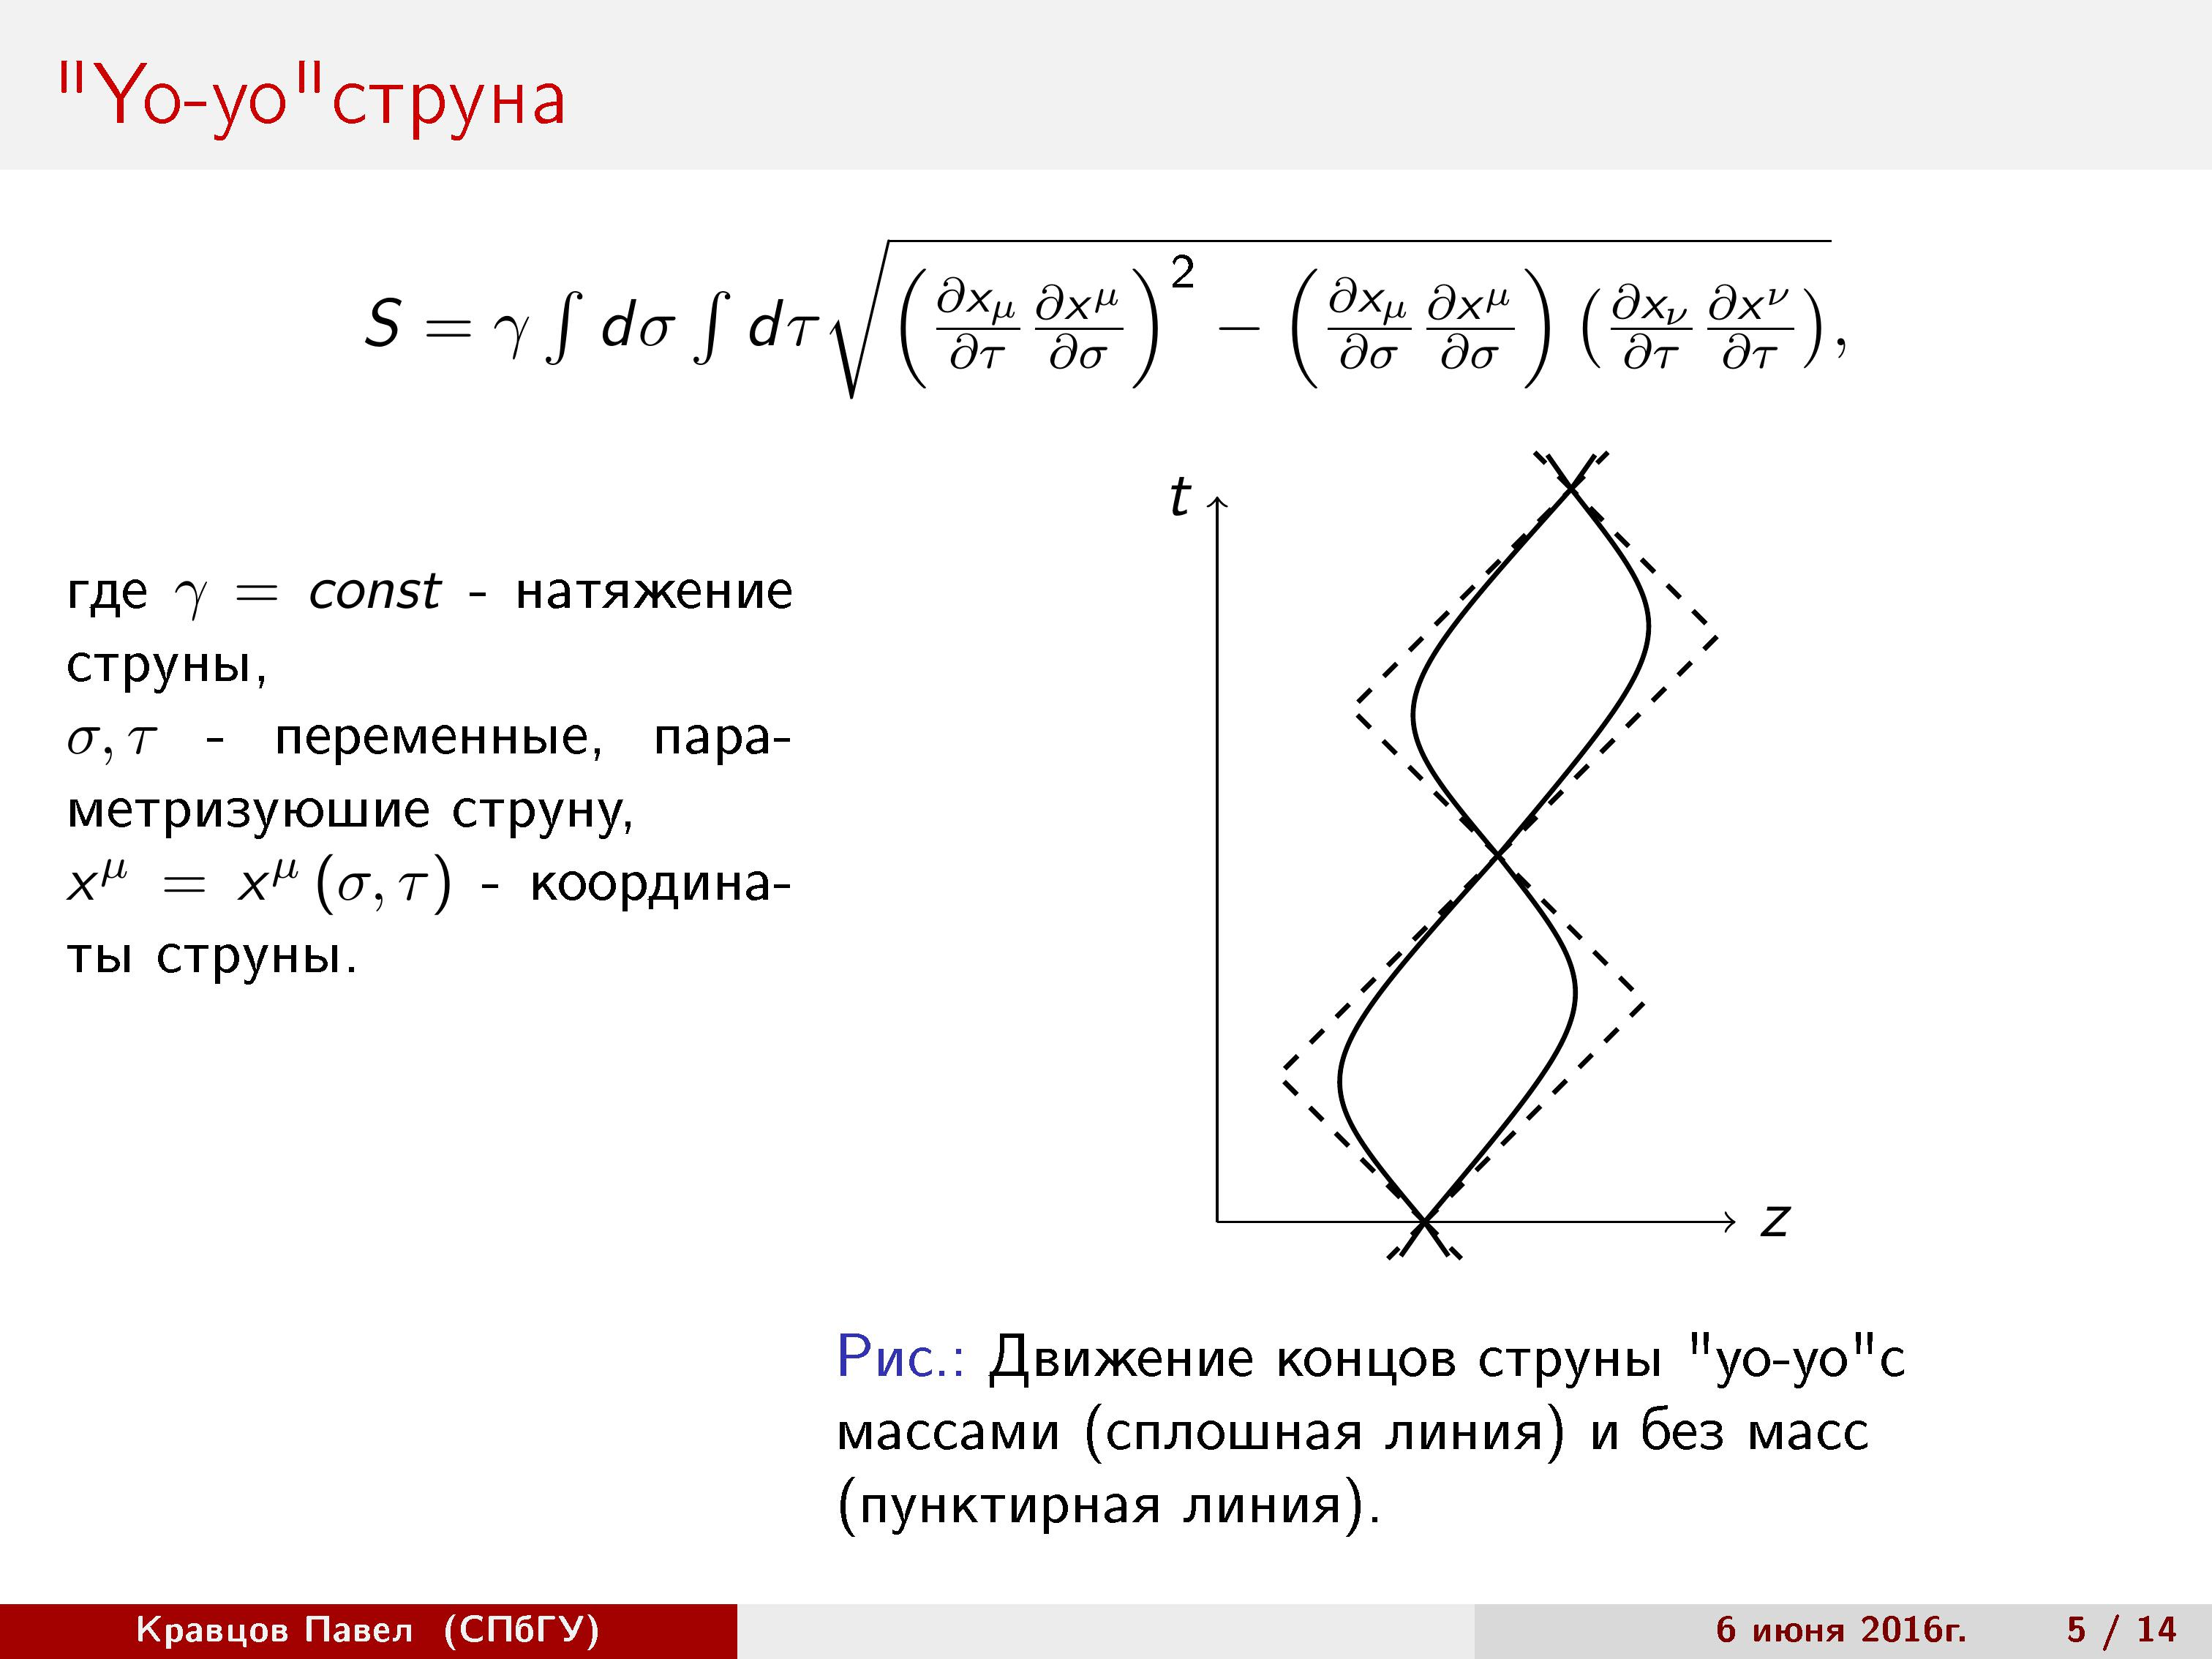
\includegraphics[width=1\linewidth]{page-05.jpg}
\end{minipage}
\begin{minipage}[h]{0.45\linewidth}
С точки зрения теоретического описания, струны - двумерный объект в пространстве времени, который описывается действием Намбу-Гото. В случае свободной струны оно выглядит так. То есть струна - это любое решение уравнений движения, соответствующее данному действию.

Как правило используется одно из простейших решений - т. н. yo-yo струна. Это решение в пространстве-времени размерности 1+1. В нем концы струны двигаются так, как показано на рисунке. Сплошные линии - движение массивных концов, пунктирные - движение безмассовых. При большой энергии кварков на концах струны они неотличимы, поэтому считаем, для простоты, что кварки на концах - безмассовые.
\end{minipage}
\line

\begin{minipage}[h]{0.35\linewidth}
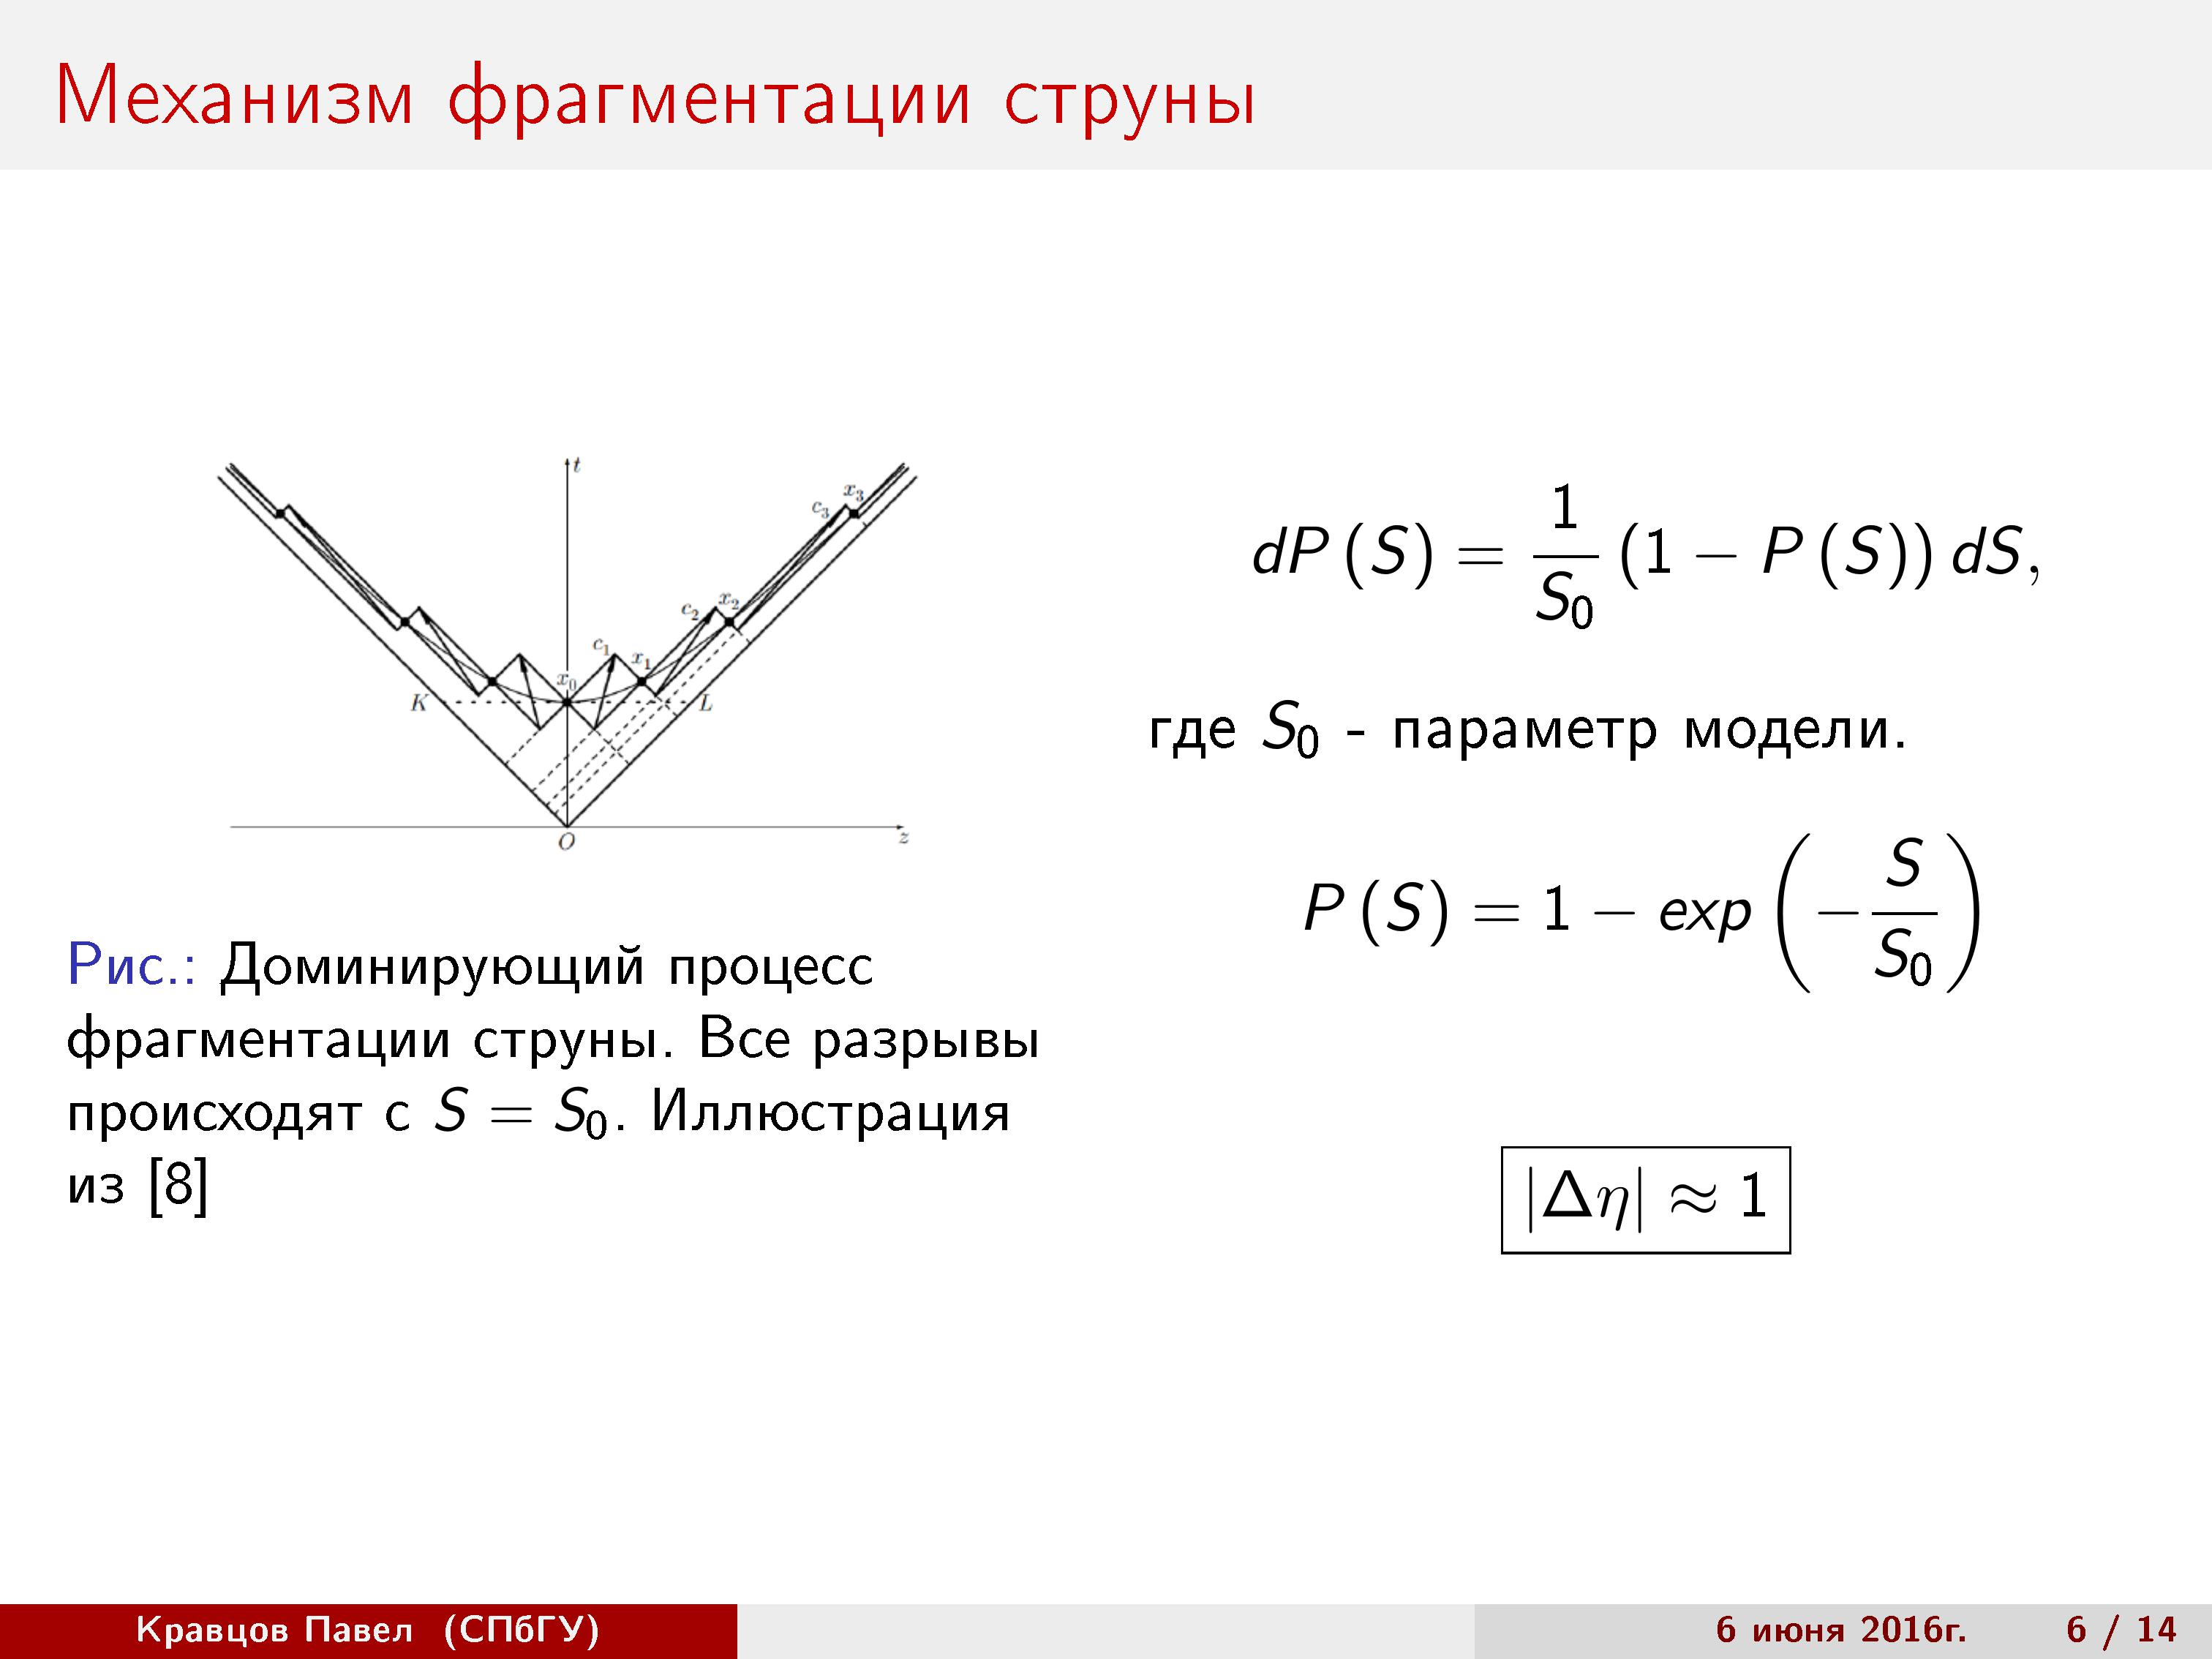
\includegraphics[width=1\linewidth]{page-06.jpg}
\end{minipage}
\begin{minipage}[h]{0.60\linewidth}
Сомо по себе действие Намбу-Гото не определяет, где и когда произойдет разрыв струны, а лишь накладывает некоторые ограничения. Поэтому придумывают феноменологические правила, удовлетворяющие этим ограничениям. Одной из них является модель Артру-Менниссиера. Для струны yo-yo она гласит, что вероятность разрыва в точке, задаваемой площадью $S$, при условии отсутствия разрывов до этого, зависит лишь от этой площади и пропорциональна ей.

Получается такой закон для вероятности разрыва. Видно, что среднее значение $S$ это $S_0$, поэтому будут преобладать процессы похожие на этот. Здесь все $S = S_0$. В работе Владимира Викторовича Вечернина показано, что в подобных процессах образуются струны равномерно распределенные по быстроте и на соседние струны-частицы приходится порядка единицы быстроты. Это главный вывод, который нам понадобиться.
\end{minipage}
\line

% 7 - 9
\newpage
$$$$
$$$$
$$$$
$$$$

\begin{minipage}[h]{0.5\linewidth}
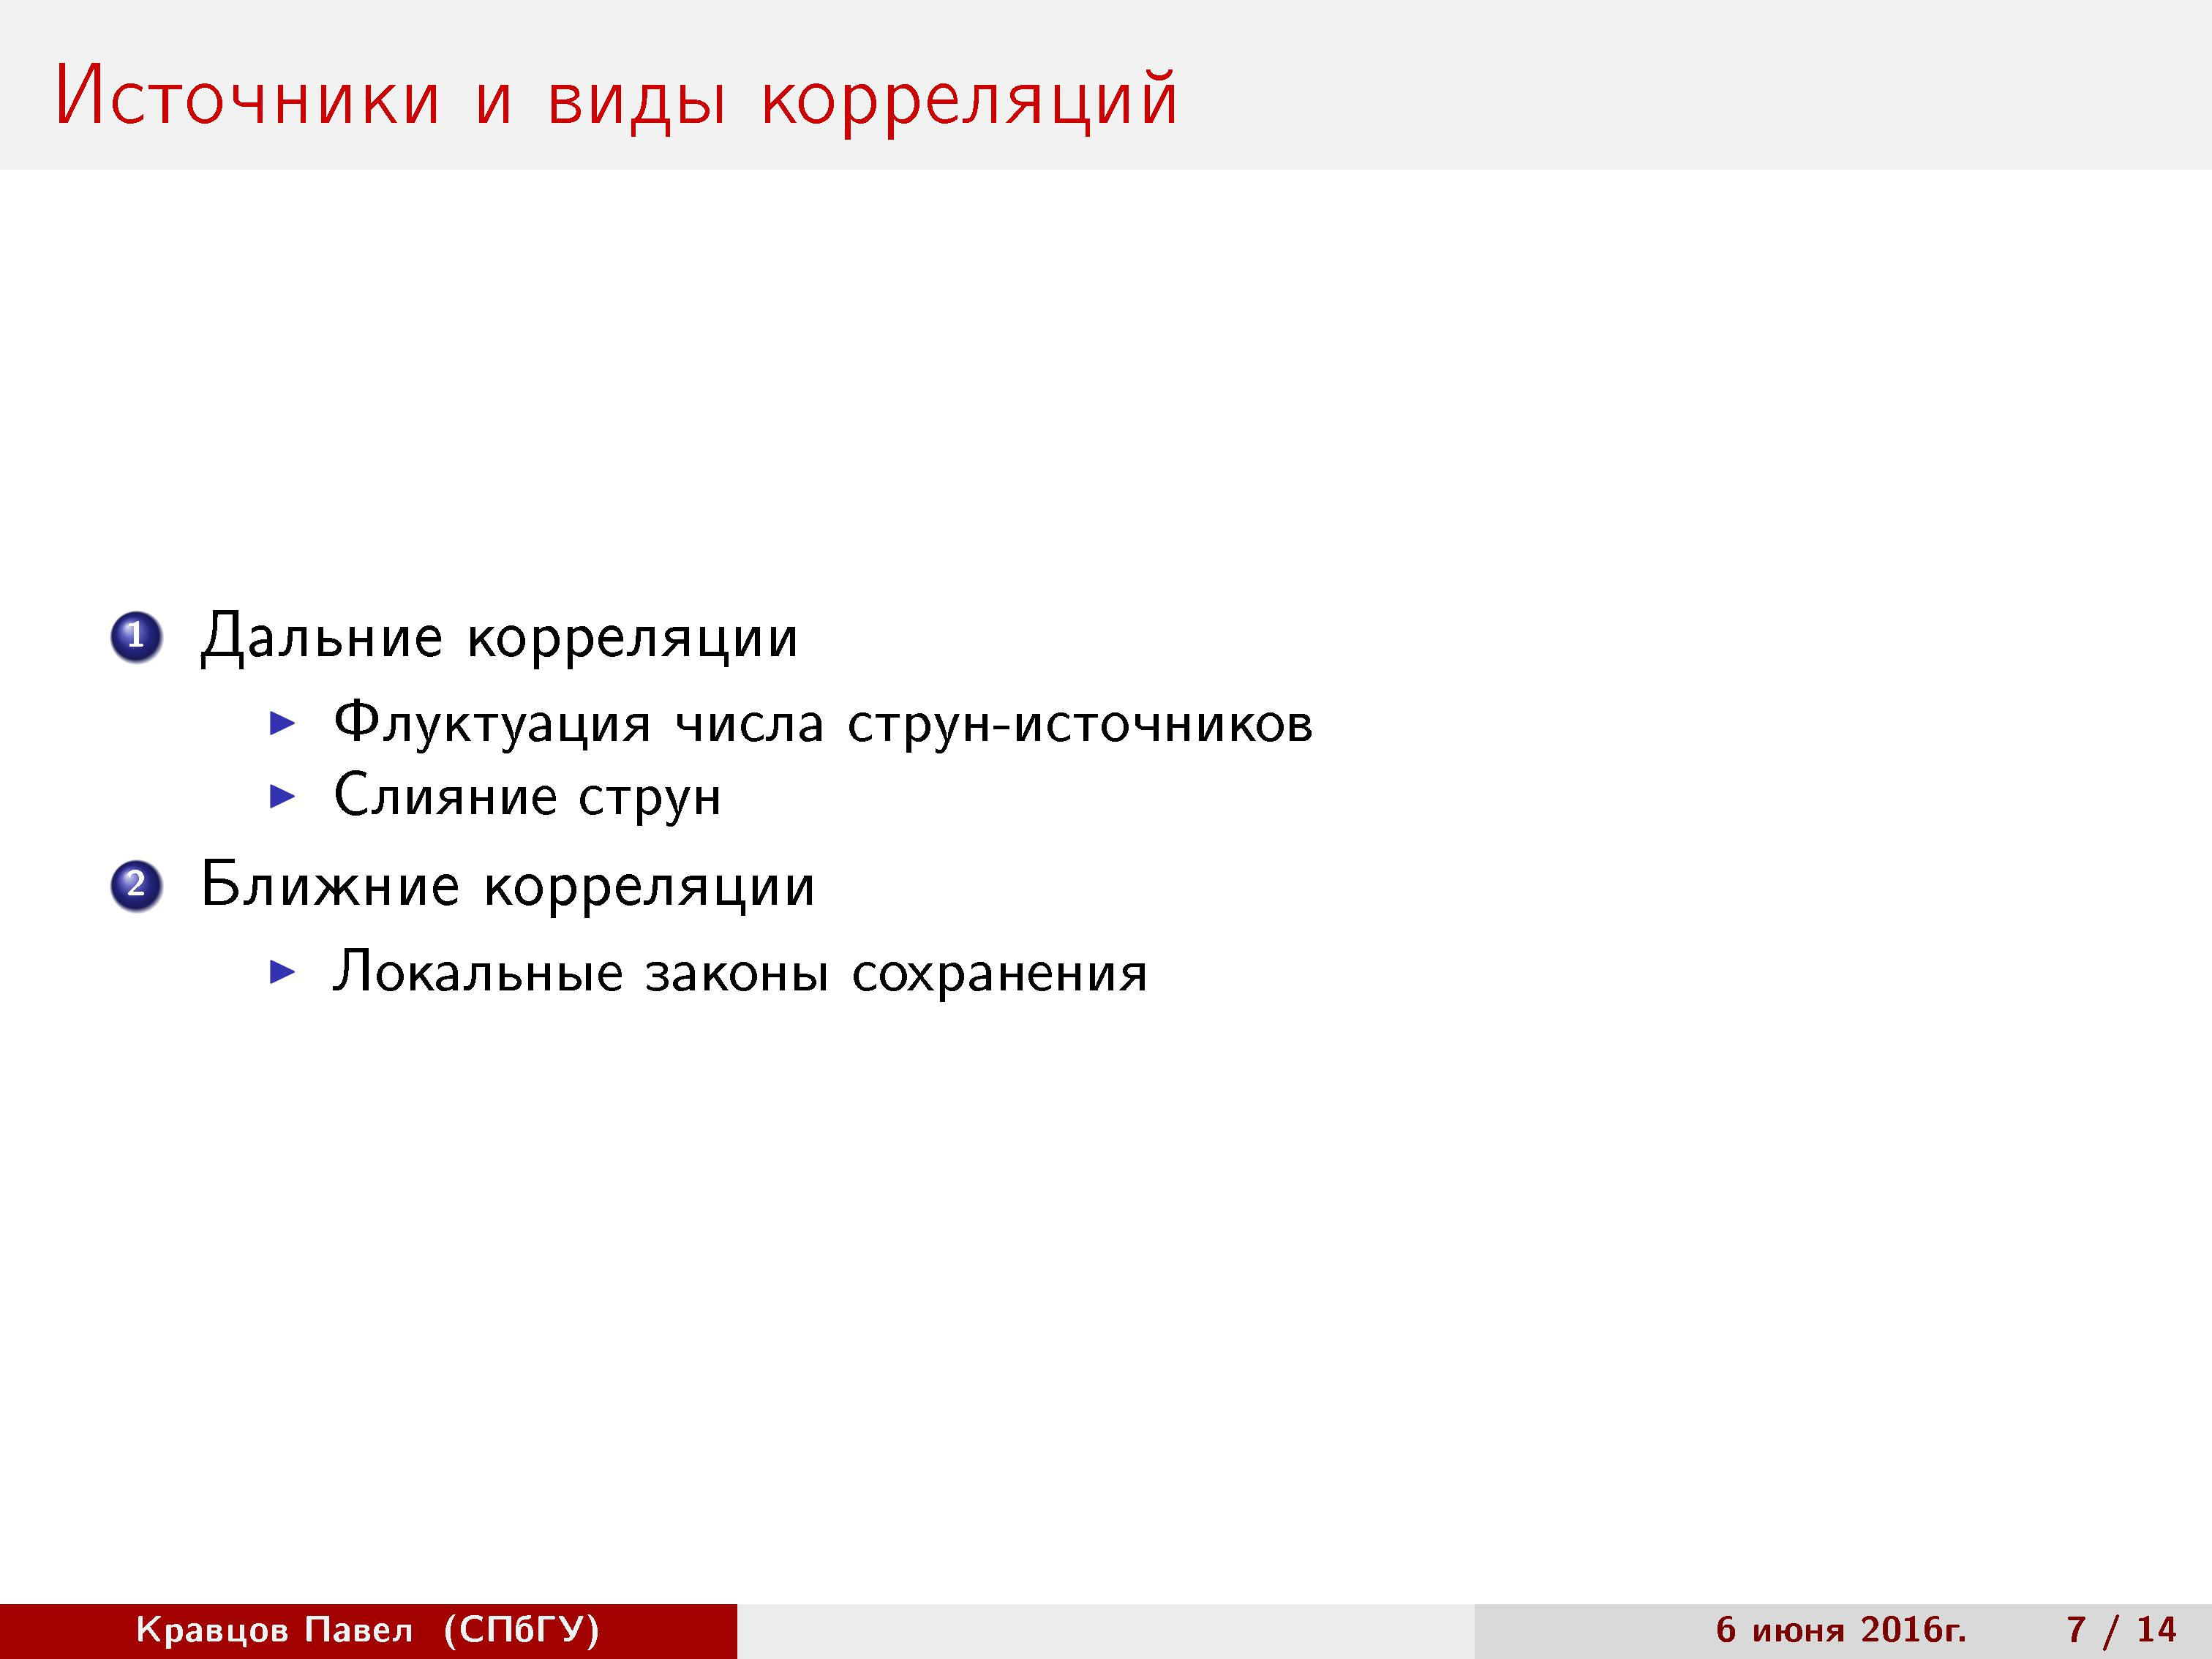
\includegraphics[width=1\linewidth]{page-07.jpg}
\end{minipage}
\begin{minipage}[h]{0.45\linewidth}
Корреляции бывают ближними и дальними. Они различаются по величине $\Delta \eta$. Дальние корреляции обусловленны флуктуацией числа струн и процессами слияния струн. Ближние корреляции обусловленны локальными законами сохранения в струнах, такими как закон сохранения импульса. В работе мы рассматриваем ближние корреляции.
\end{minipage}
\line

\begin{minipage}[h]{0.5\linewidth}
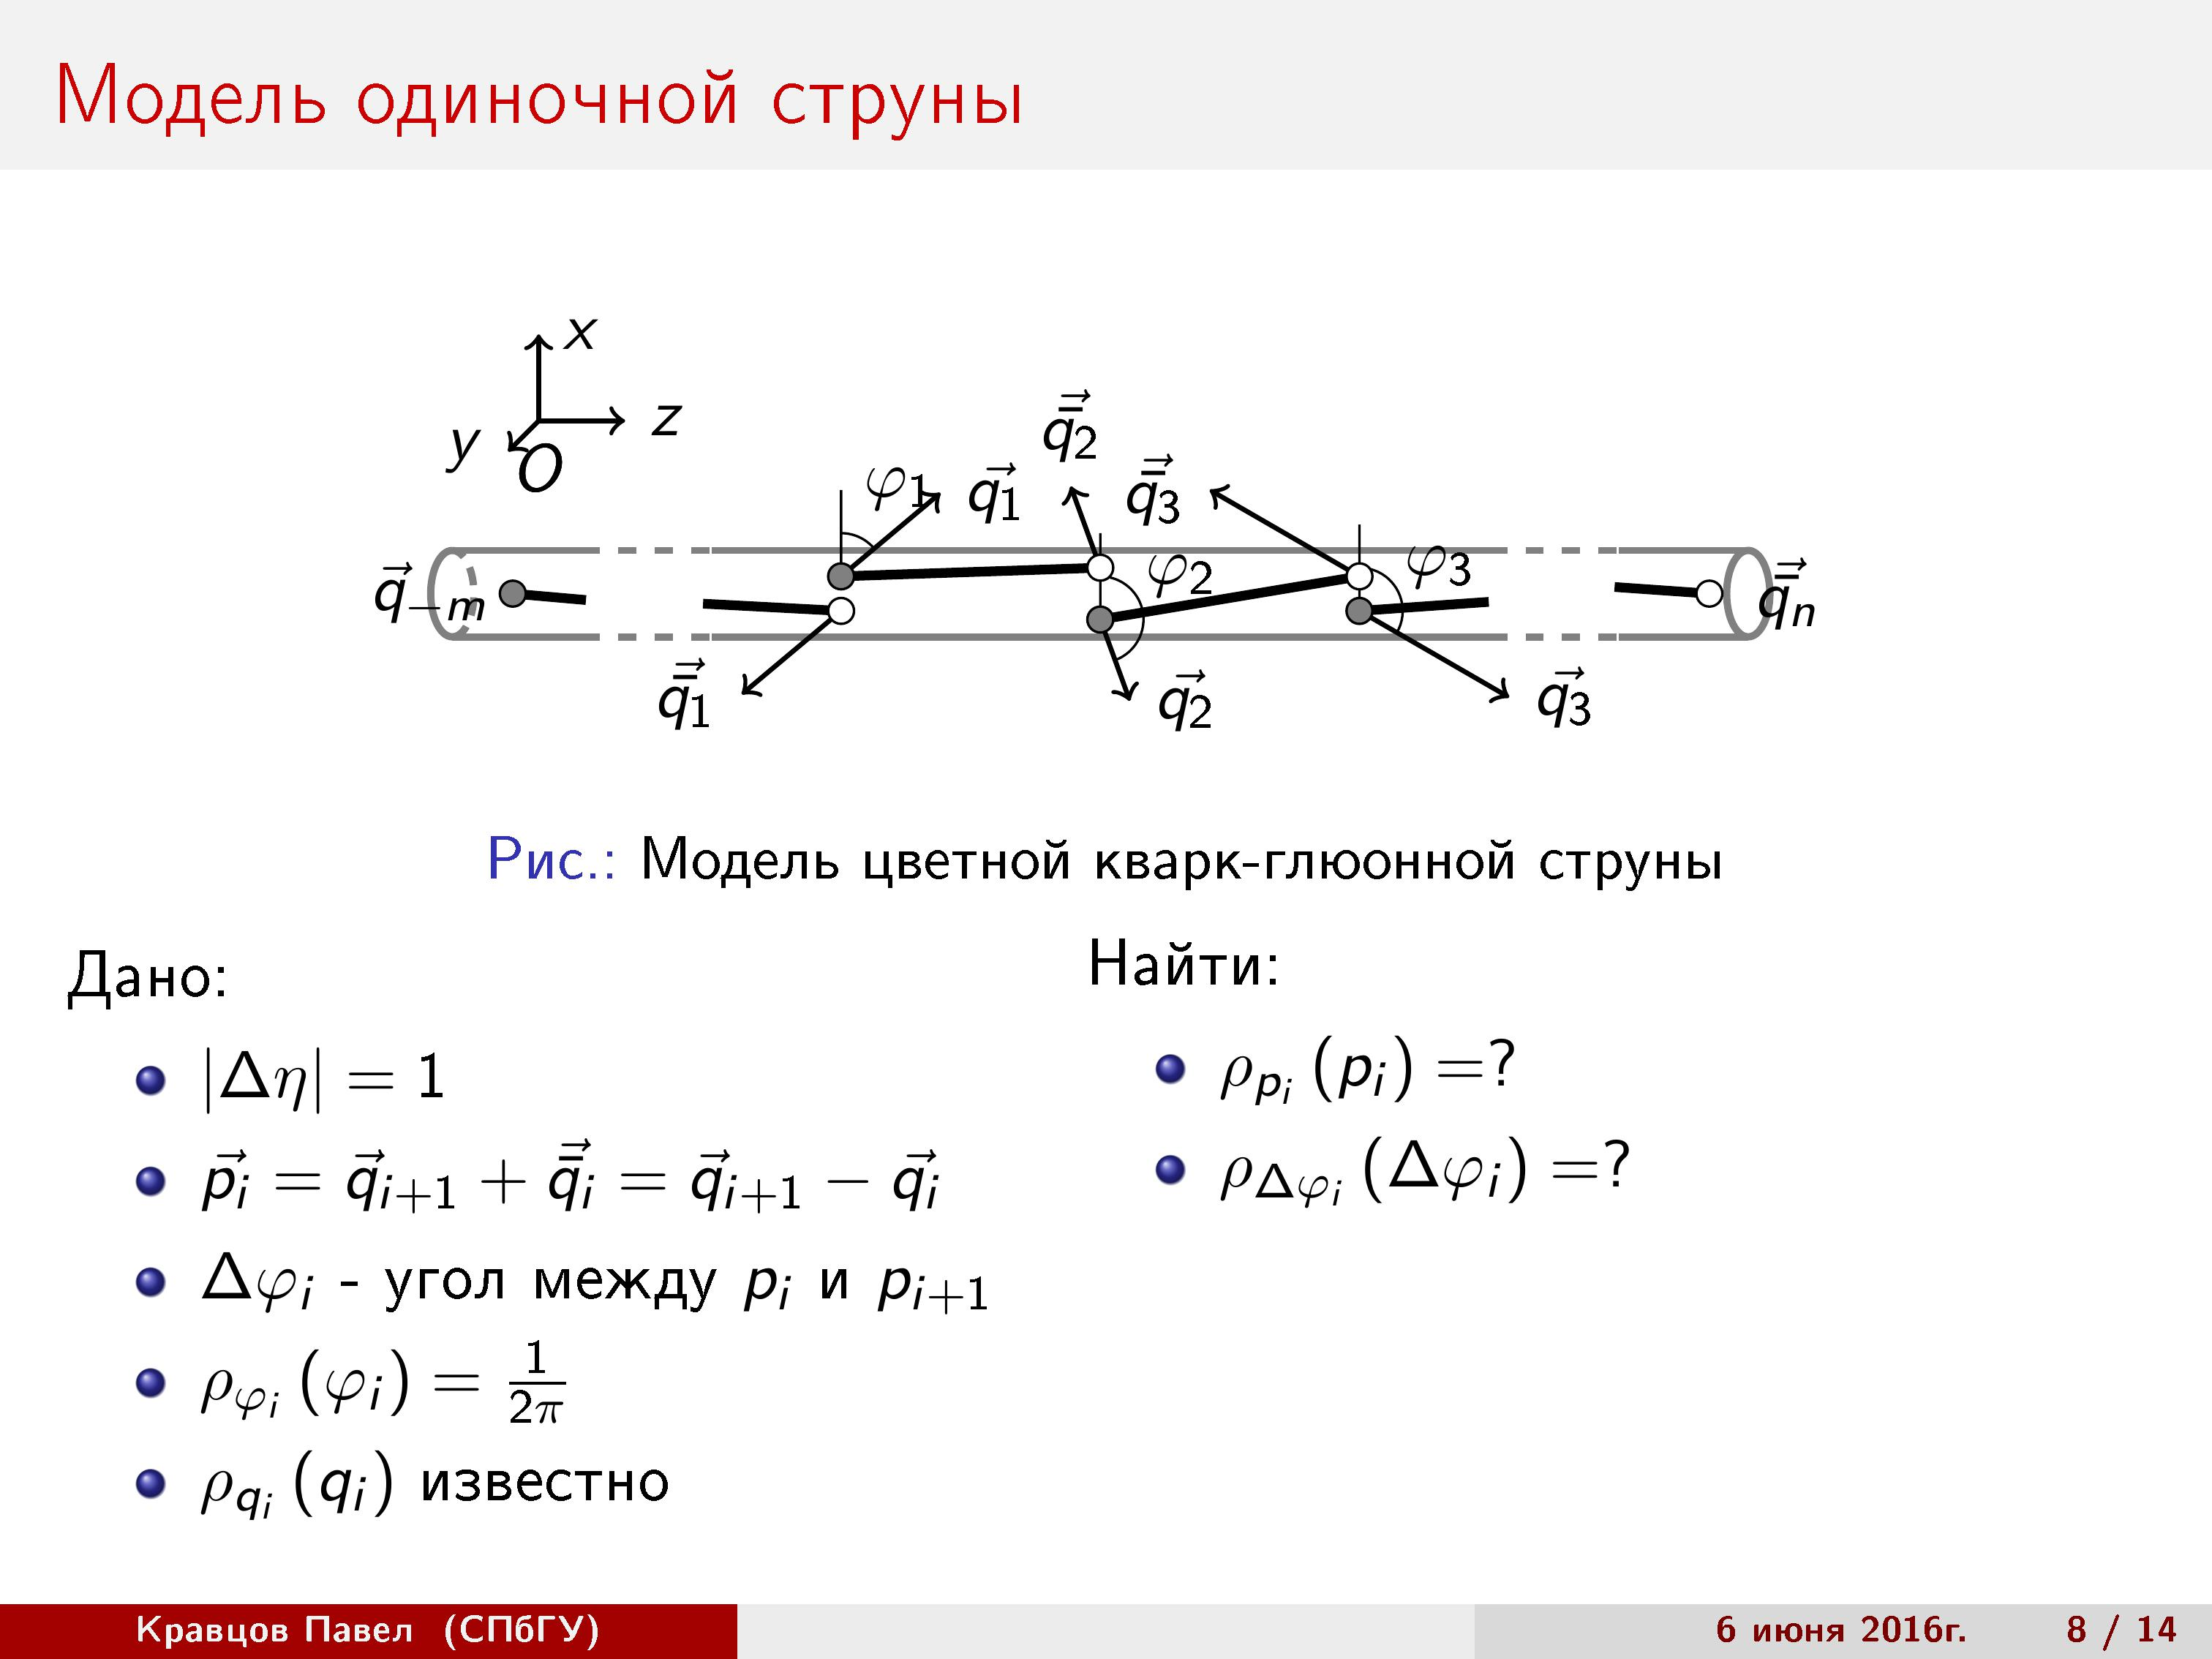
\includegraphics[width=1\linewidth]{page-08.jpg}
\end{minipage}
\begin{minipage}[h]{0.45\linewidth}
Формализуем нашу модель. Есть расширяющаяся струна. Она рвется в некоторых точках, что означает рождение пар кварк-антикварк в этих точках и обрзованию новых струн. Соседние струны отличаются на единицу по быстроте. $q_i, \bar{q_i}$ поперечные импульсы кварков и антикварков соответственно. $\phi_i$ угол между осью x и направлением поперечного импульса кварков. Импульс мезонов - сумма  $\vec{q}_{i+1} + \vec{\bar{q_i}}$ равная, из-за закона сохранения импульса $\vec{q}_{i+1} - \vec{q_i}$. $\Delta \phi$ - угол между поперечными импульсами соседних частиц. Мы считаем, что $phi_i$ распределенно равномерно, а распределение поперечного импульса кварка нам известно. Из них мы находим распределение по поперечному импульсу образовавшихся мезонов и распределение по углу разлета.
\end{minipage}
\line

\begin{minipage}[h]{0.5\linewidth}
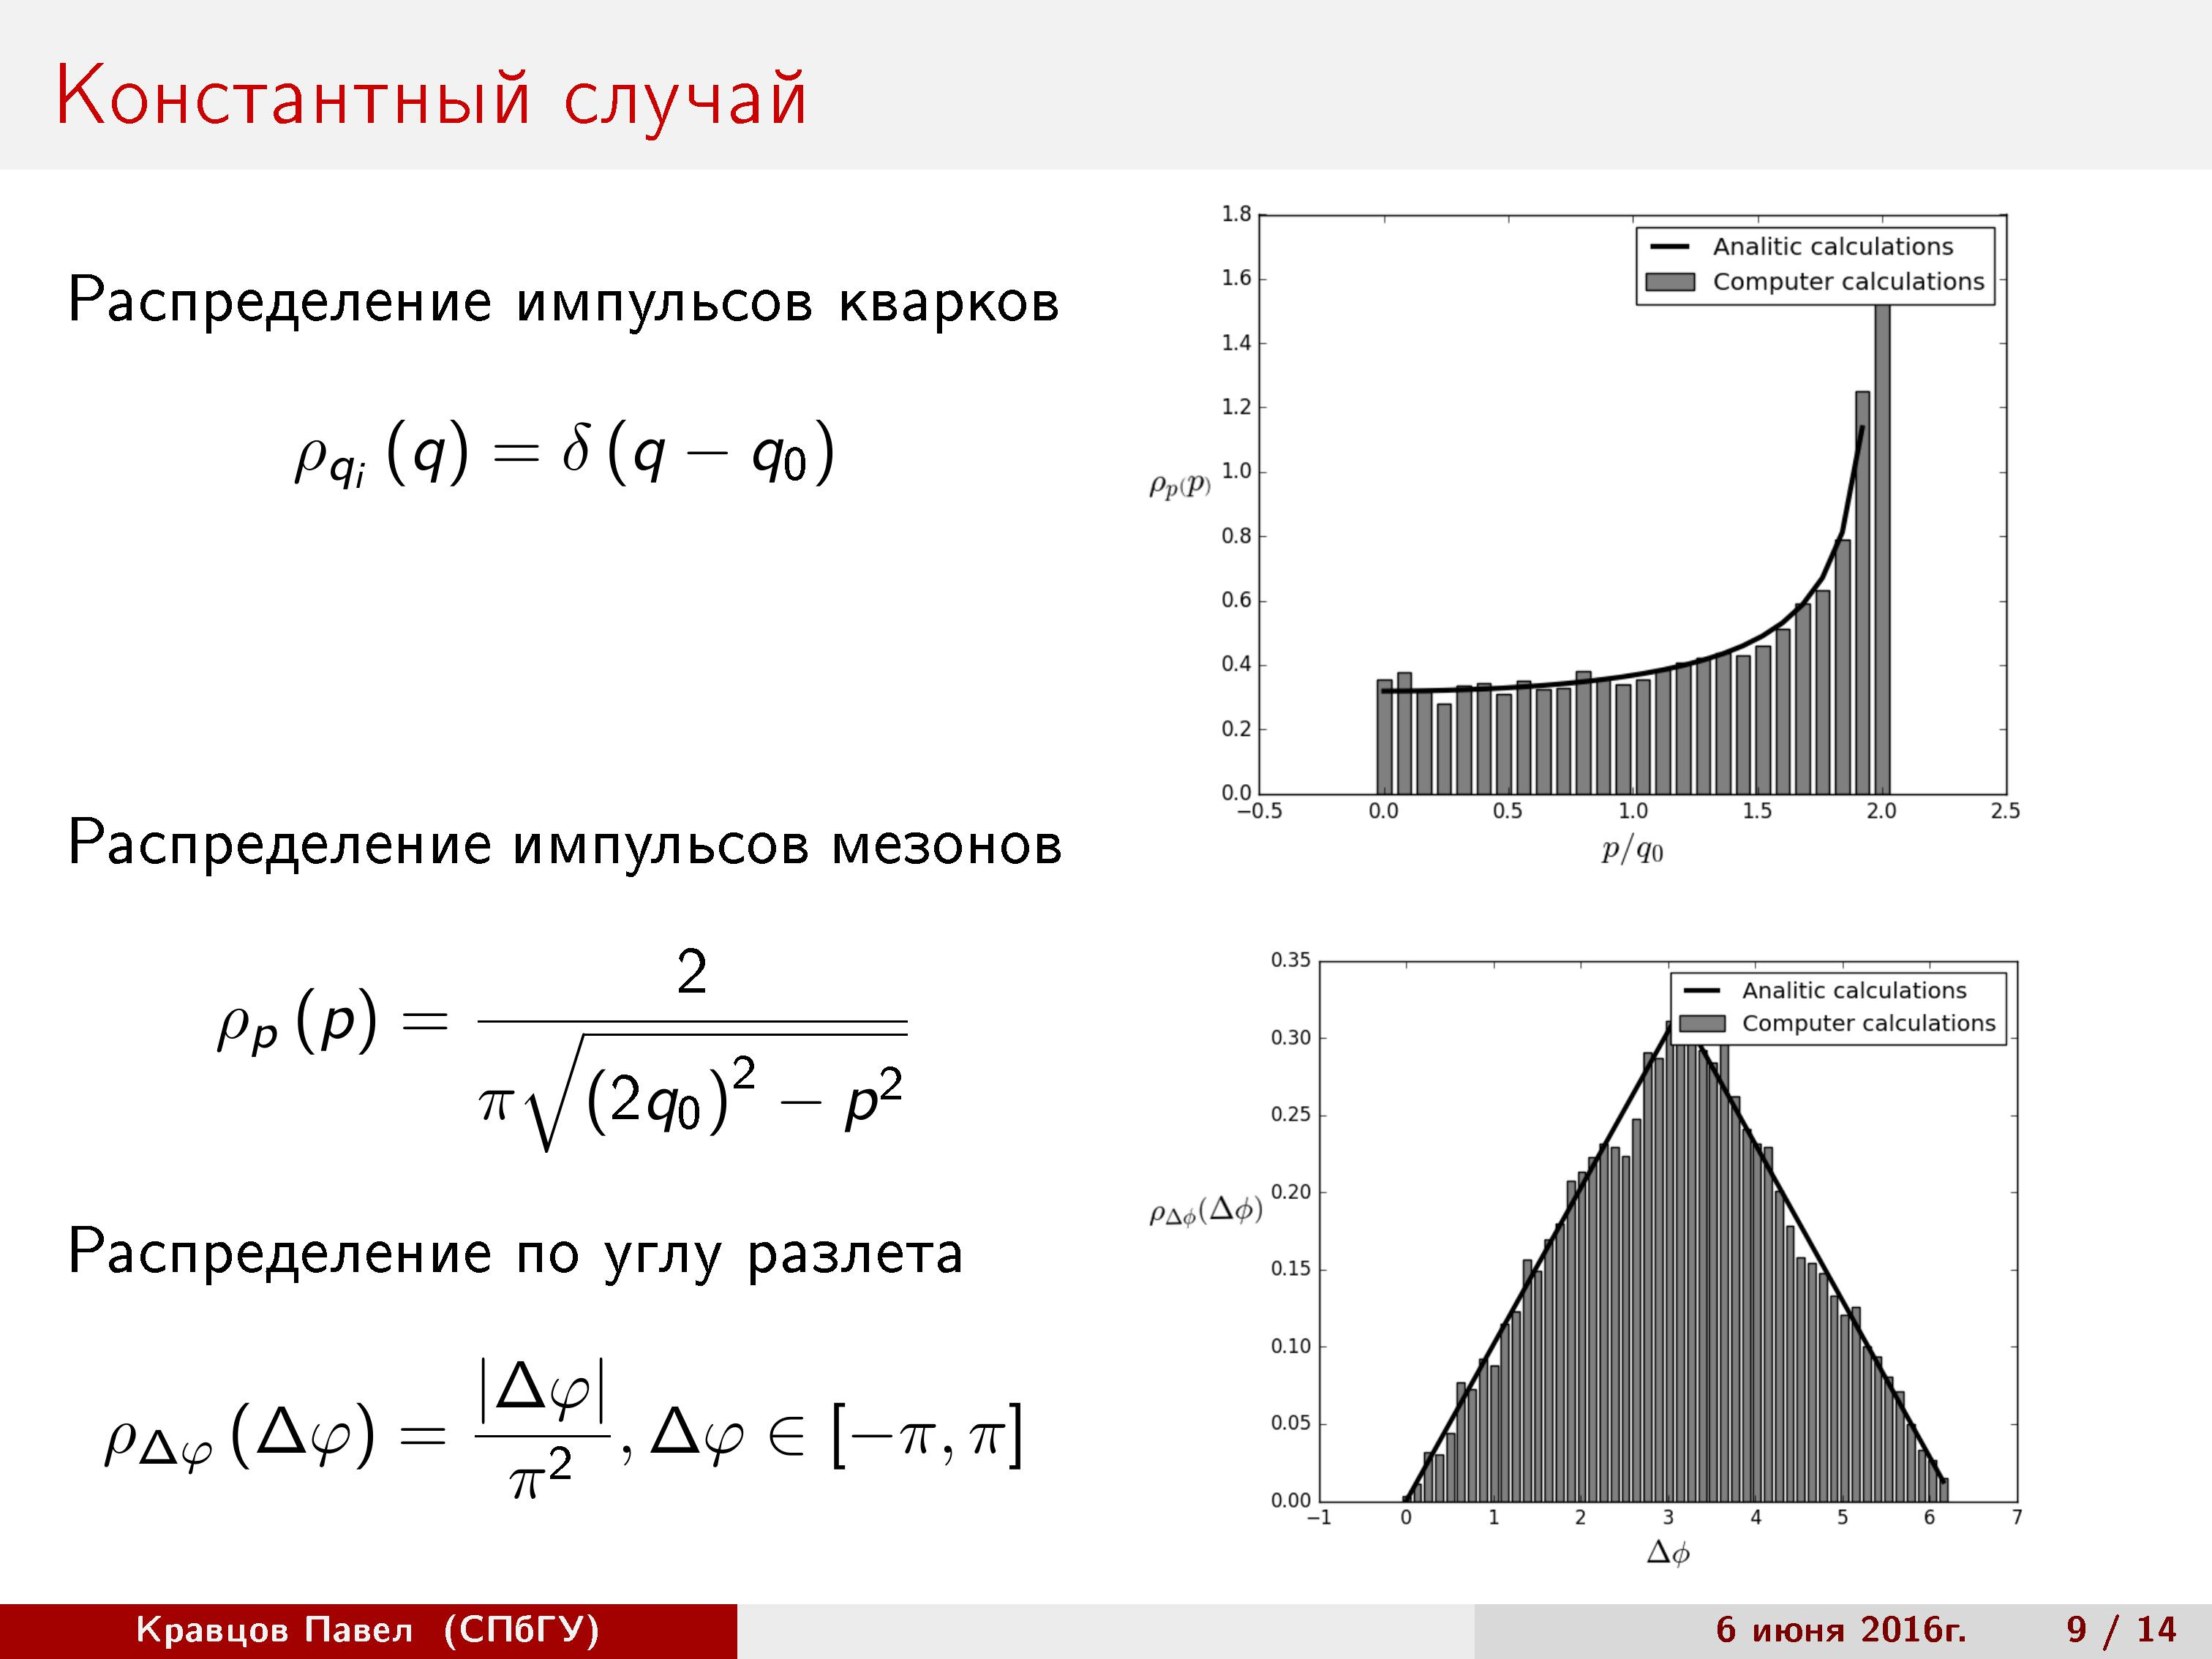
\includegraphics[width=1\linewidth]{page-09.jpg}
\end{minipage}
\begin{minipage}[h]{0.45\linewidth}
Мы рассматривали 2 случая для распределения кварков. Первый случай, когда величины поперечных импульсов все равны $q_0$. Тогда был получены данные выражения для распределений. Здесь опушен индекс i, т. к. от него ничего не зависит. Также была написана программа для проверки этих выражений методом Монте-Карло. Результаты представленны на графике. Для угла разлета мы видим пик в точке $\Delta \phi = \pi$.
\end{minipage}
\line

% 10 - 12
\newpage
$$$$
$$$$
$$$$
$$$$

\begin{minipage}[h]{0.5\linewidth}
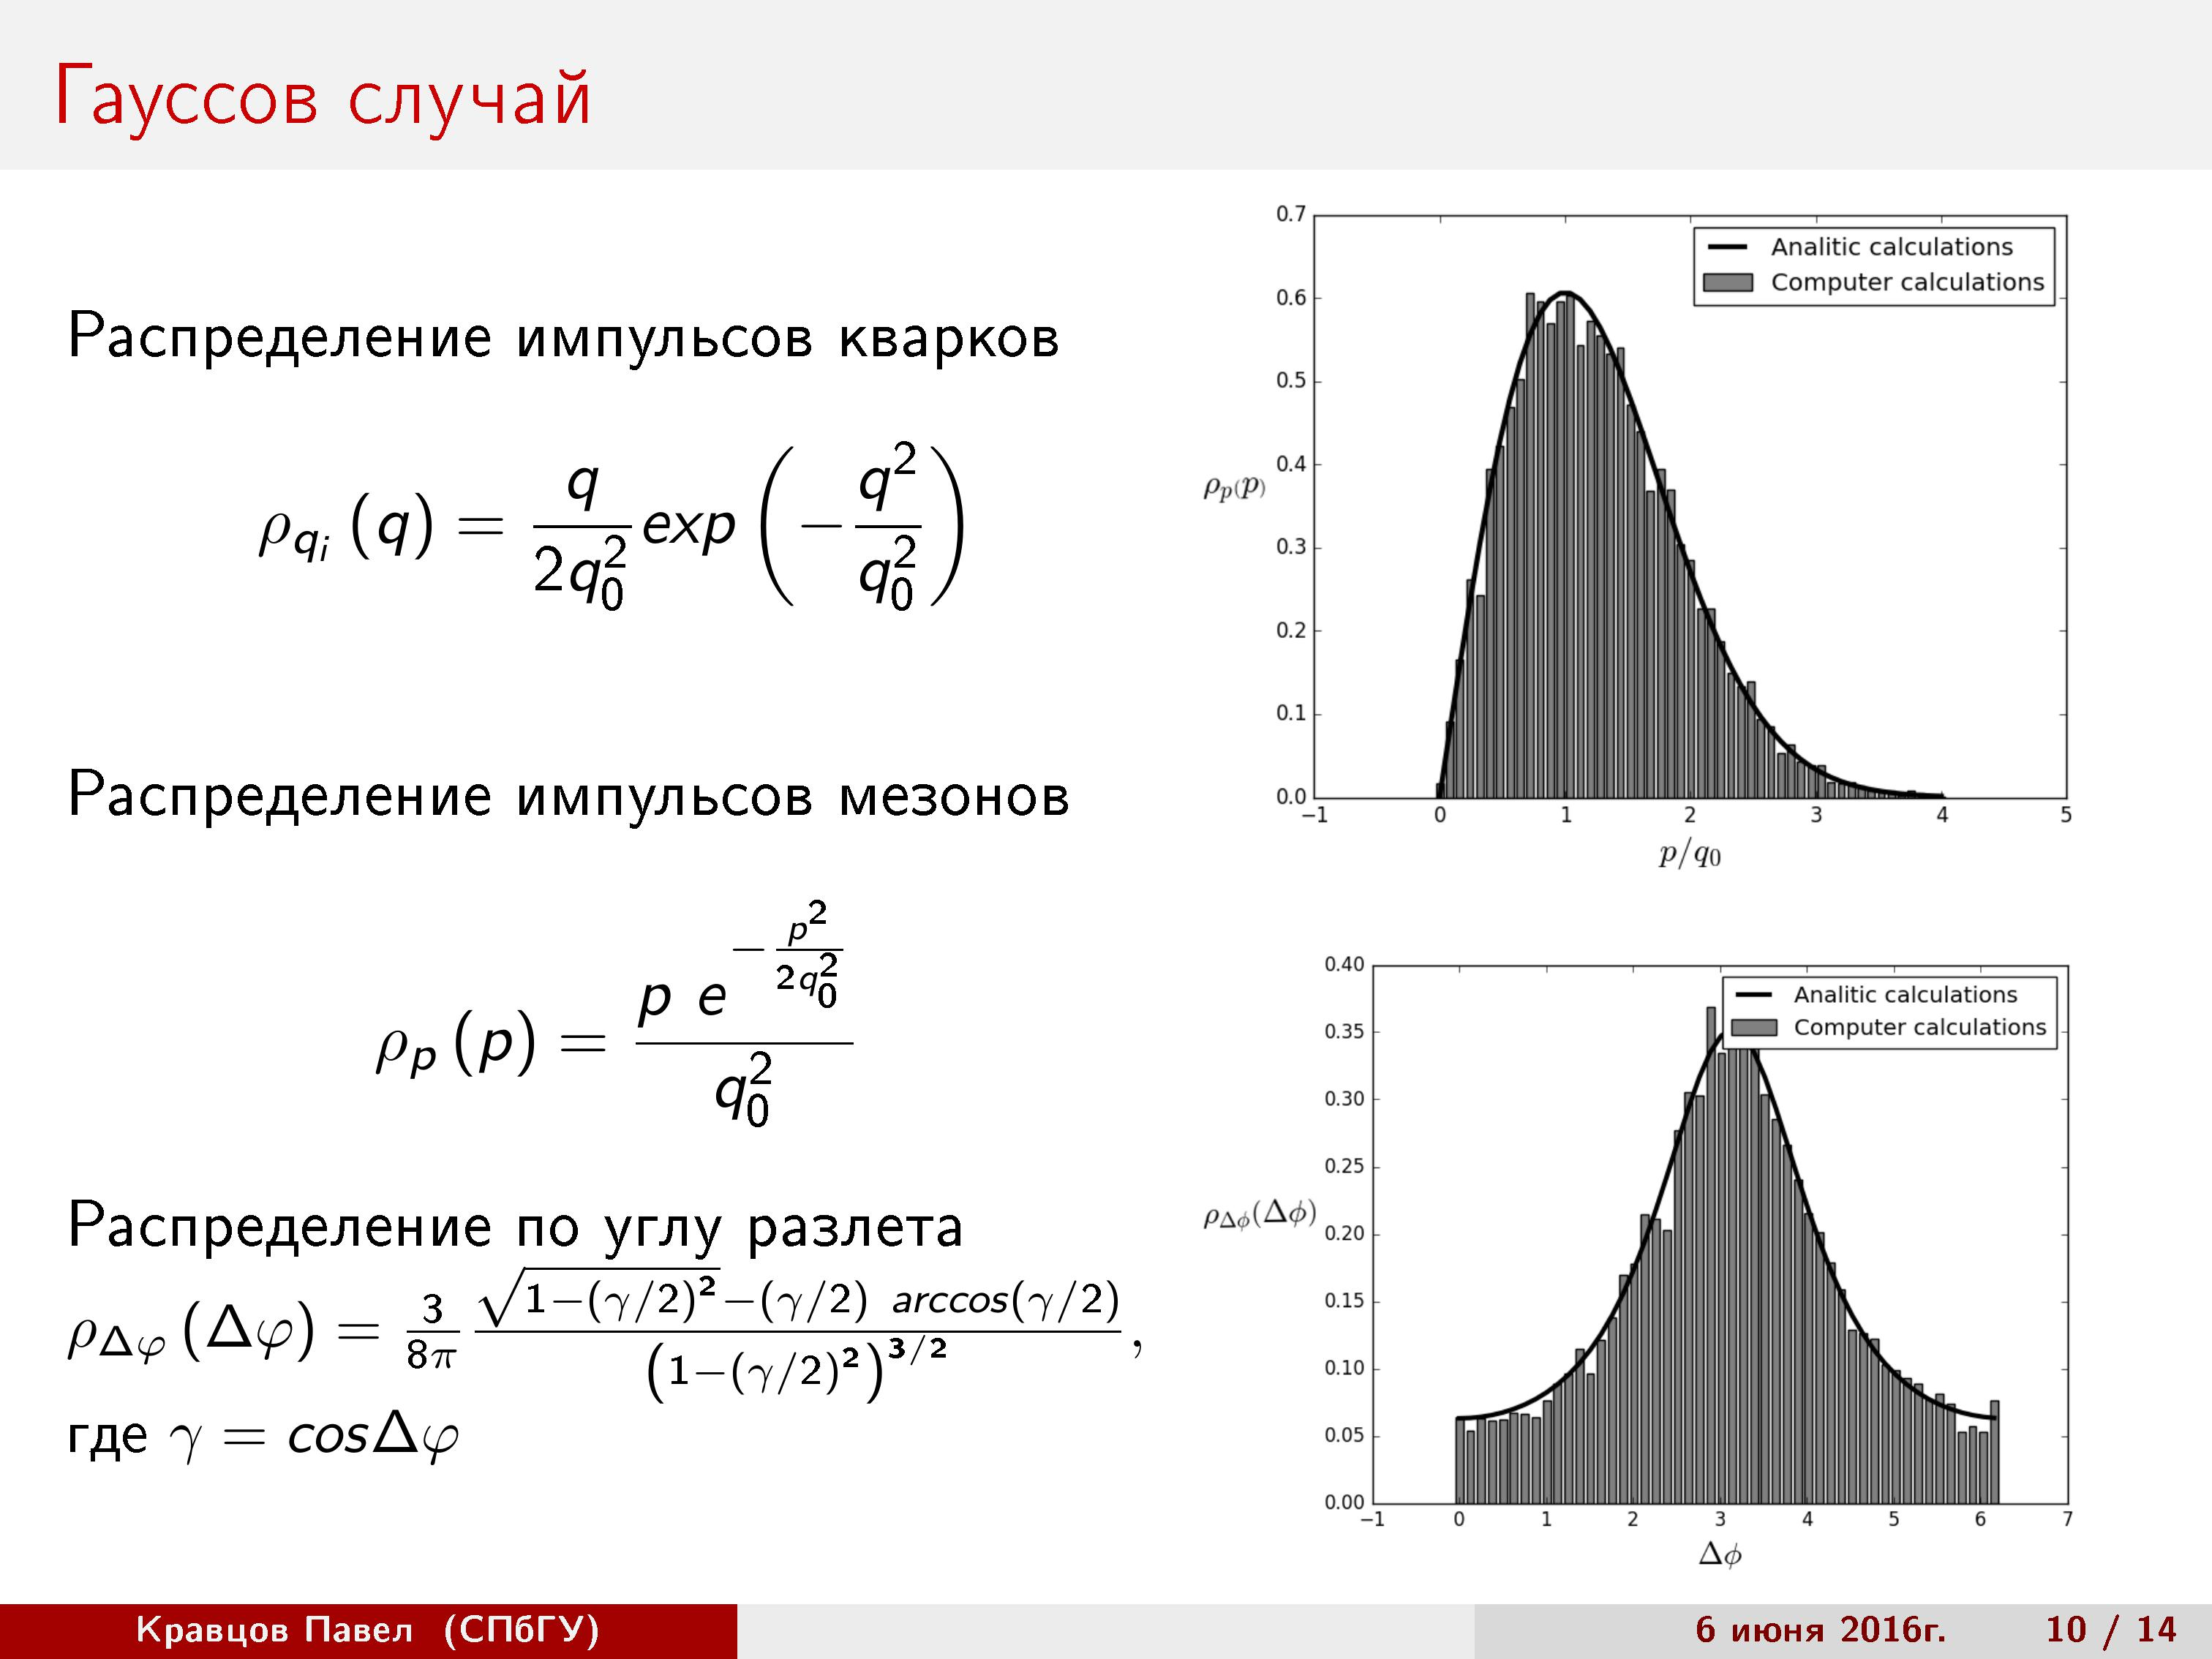
\includegraphics[width=1\linewidth]{page-10.jpg}
\end{minipage}
\begin{minipage}[h]{0.45\linewidth}
Второй случай, это распределение по гауссу. Были полученны следующие распределения. Здесь тоже имеется пик в точке $\Delta \phi = \pi$.
\end{minipage}
\line

\begin{minipage}[h]{0.3\linewidth}
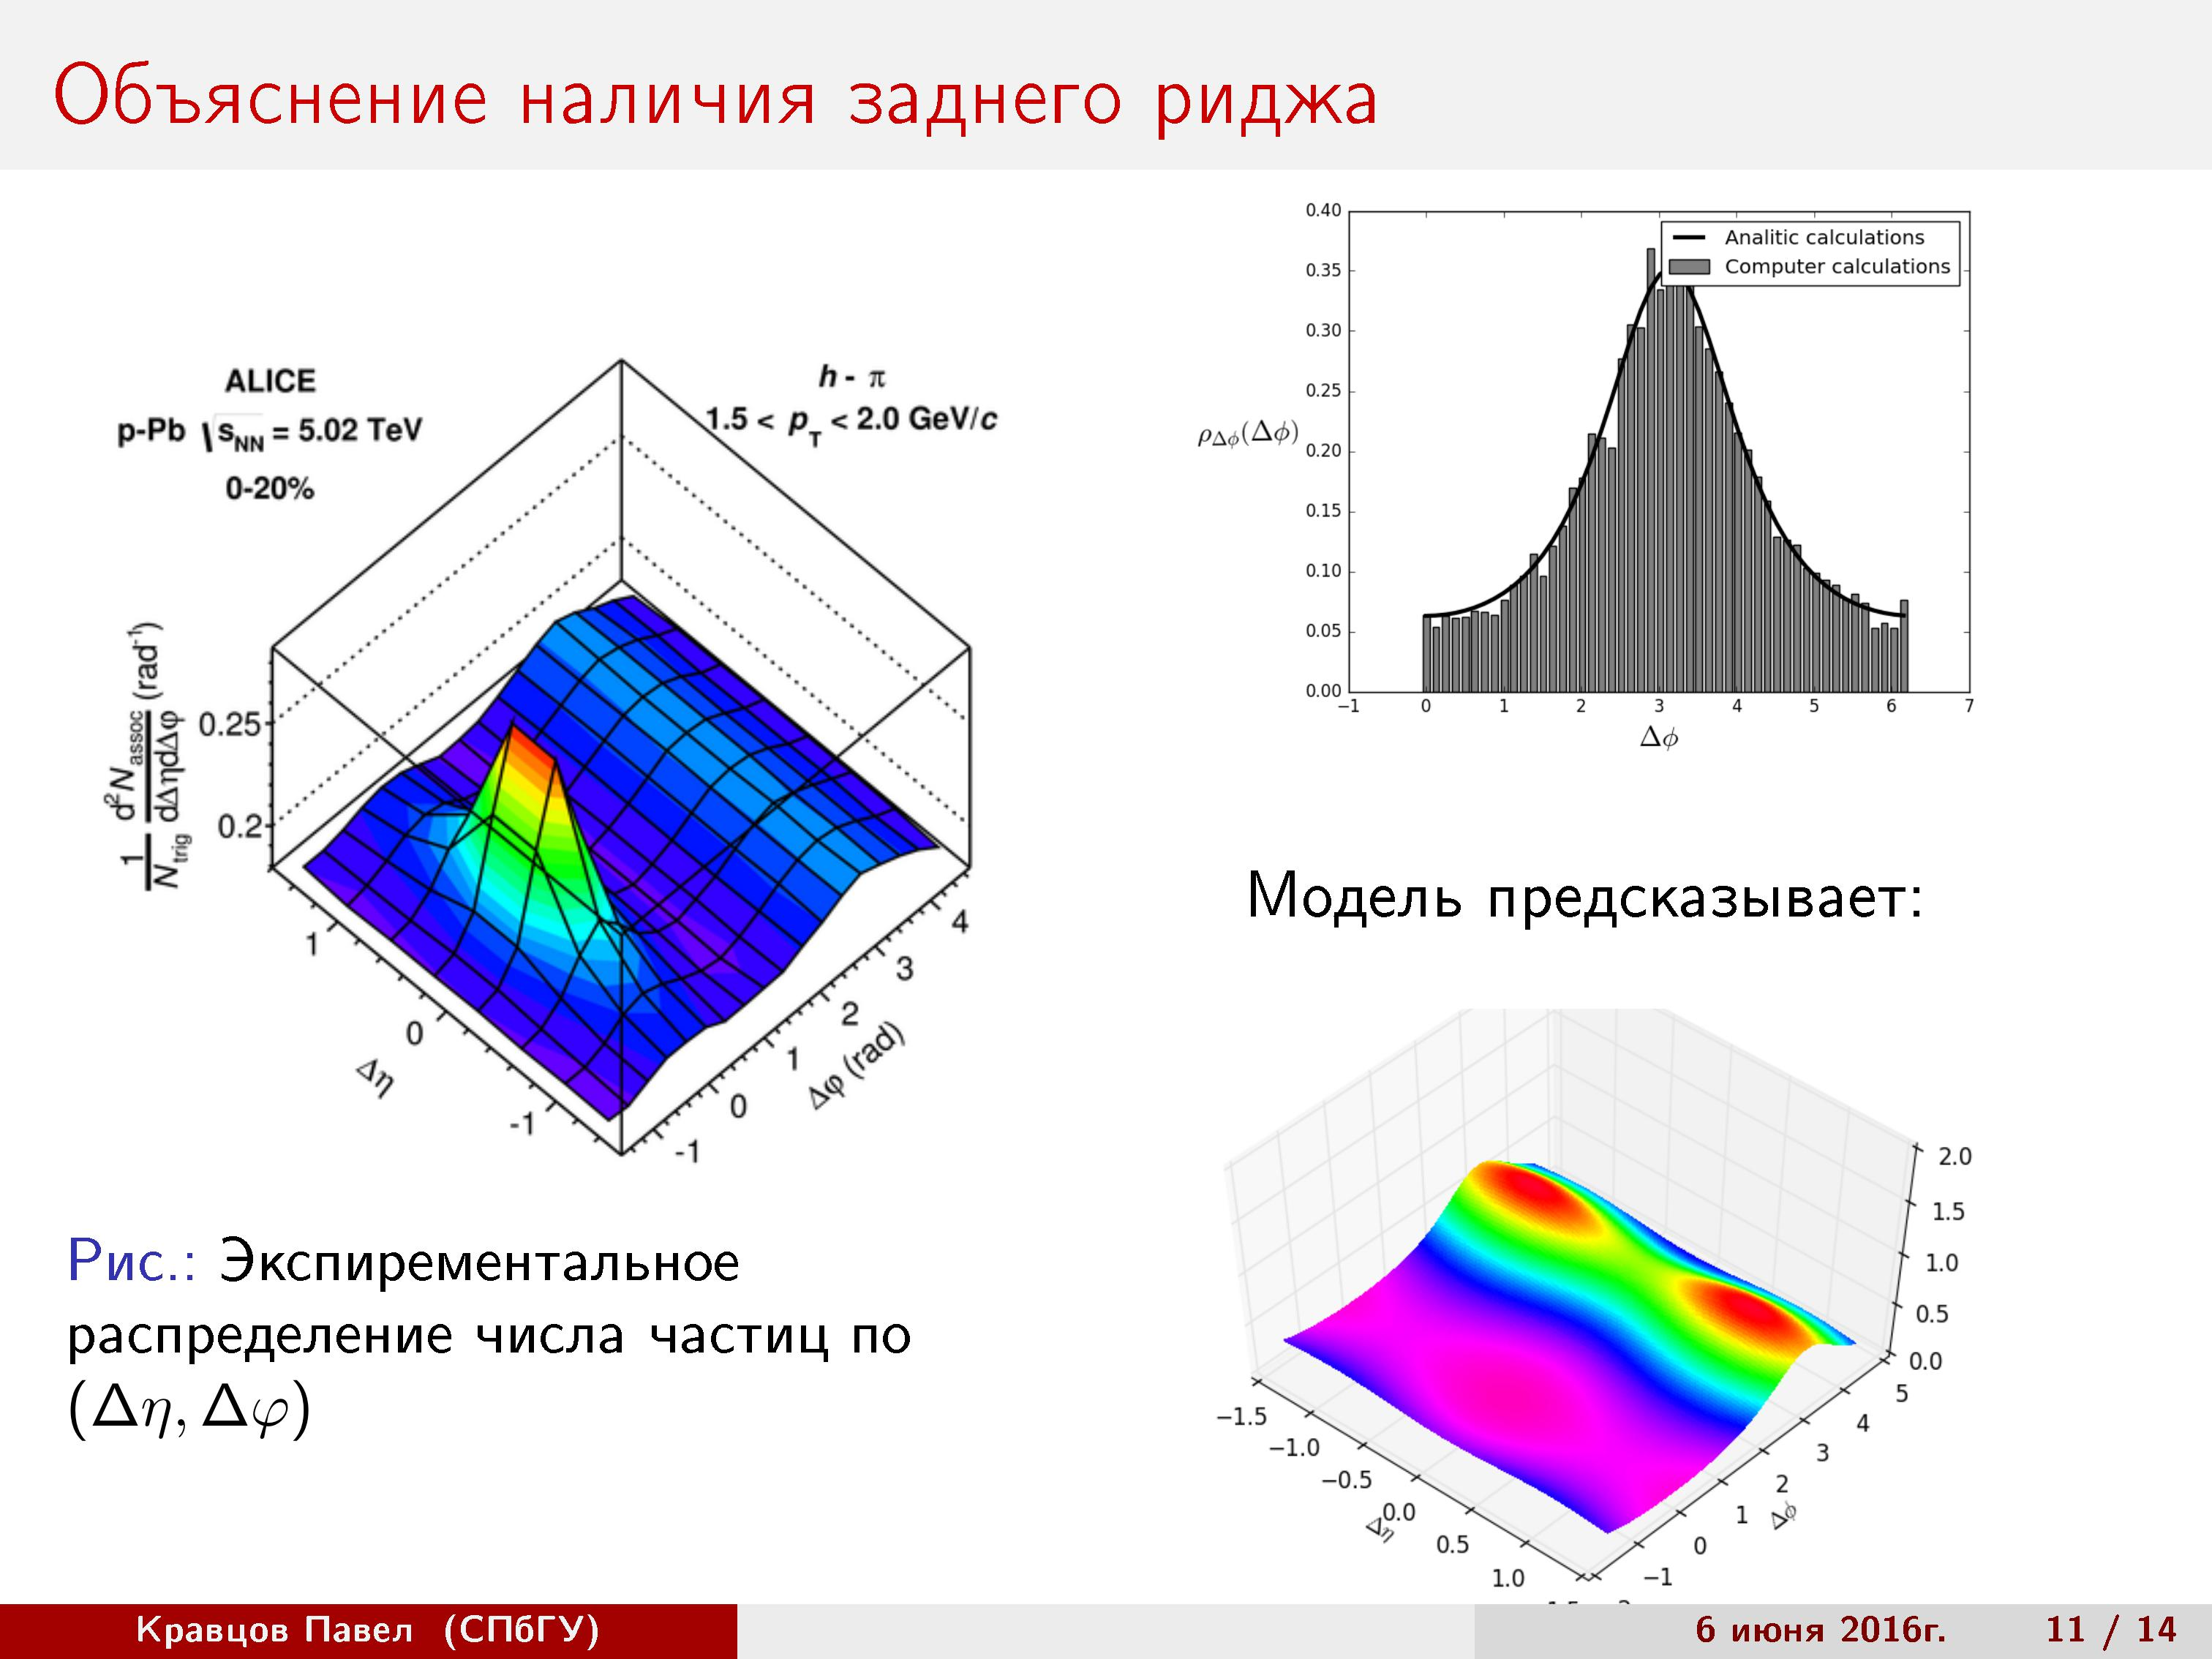
\includegraphics[width=1\linewidth]{page-11.jpg}
\end{minipage}
\begin{minipage}[h]{0.65\linewidth}
Вернемся к цели работы. Сначала несколько слов о переднем пике. 
Он говорит о том, что образуется много пар частиц летящих в одну сторону с одной быстротой. Это объясняется тем, что в после фрагментации образуетются не только частицы с основным состоянием, но и частицы с резонансным состоянием. Подобные резонансы до улавливания детекторами сами распадаются на две и более стабильные частицы. Детекторы регистрируют именно эти стабильные частицы, которые разумеется будут иметь схожие быстроты и направления.

В нашей модели появляется пик с центром $\Delta \phi = \pi$. Для  функции распределения (на рис. \ref{main}), так как в среднем на одну частицу приходится одна единица быстроты и частицы от соседних струн в среднем разделены интервалом $\abs{\Delta \eta} = 1$, это означает появление двух холмов с центрами в точках $(\Delta \phi , \Delta \eta) = (\pi, -1)$ и $(\Delta \phi , \Delta \eta) = (\pi, 1)$. На рисунке мы видим их сильно "размазаными" по быстроте, то есть именно они и формируют задний ридж.
\end{minipage}
\line

\begin{minipage}[h]{0.5\linewidth}
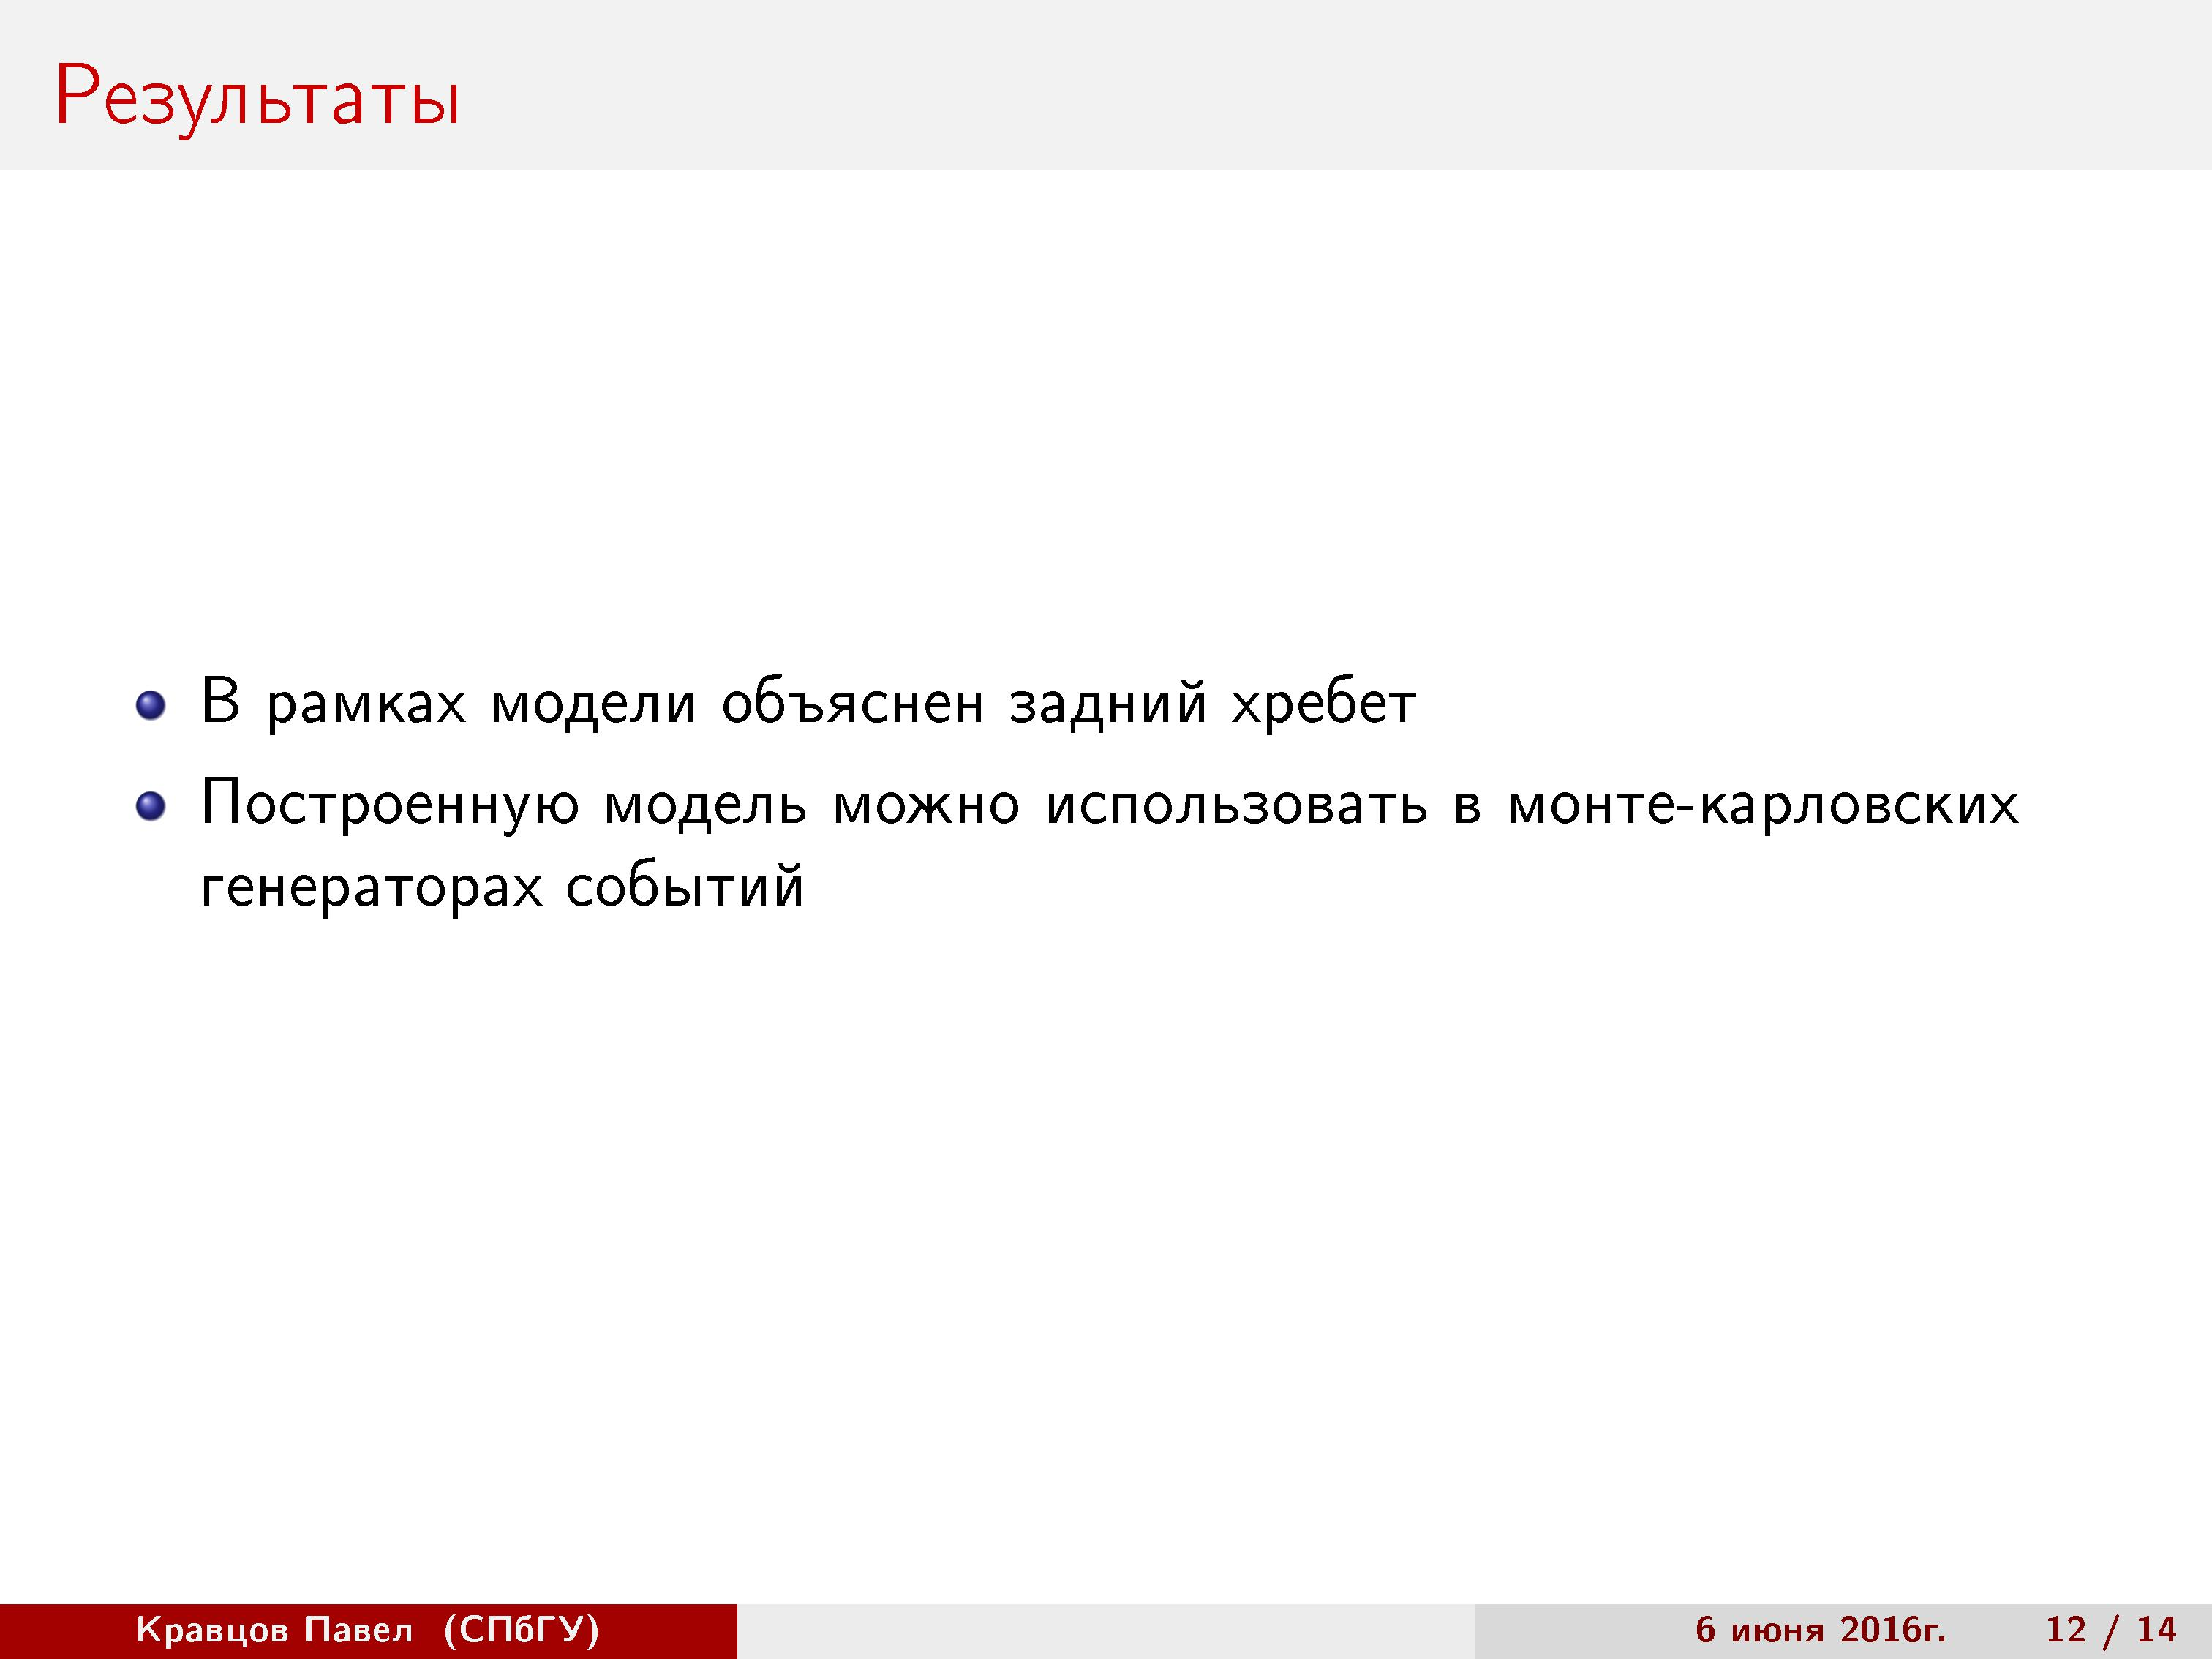
\includegraphics[width=1\linewidth]{page-12.jpg}
\end{minipage}
\begin{minipage}[h]{0.45\linewidth}
Прочитать слайд
\end{minipage}
\line
\end{document}